% Graphic for TeX using PGF
% Title: /home/tassia/AppRecommender/fig/app_rec.dia
% Creator: Dia v0.97.1
% CreationDate: Tue May 31 17:00:05 2011
% For: tassia
% \usepackage{tikz}
% The following commands are not supported in PSTricks at present
% We define them conditionally, so when they are implemented,
% this pgf file will use them.
\ifx\du\undefined
  \newlength{\du}
\fi
\setlength{\du}{15\unitlength}
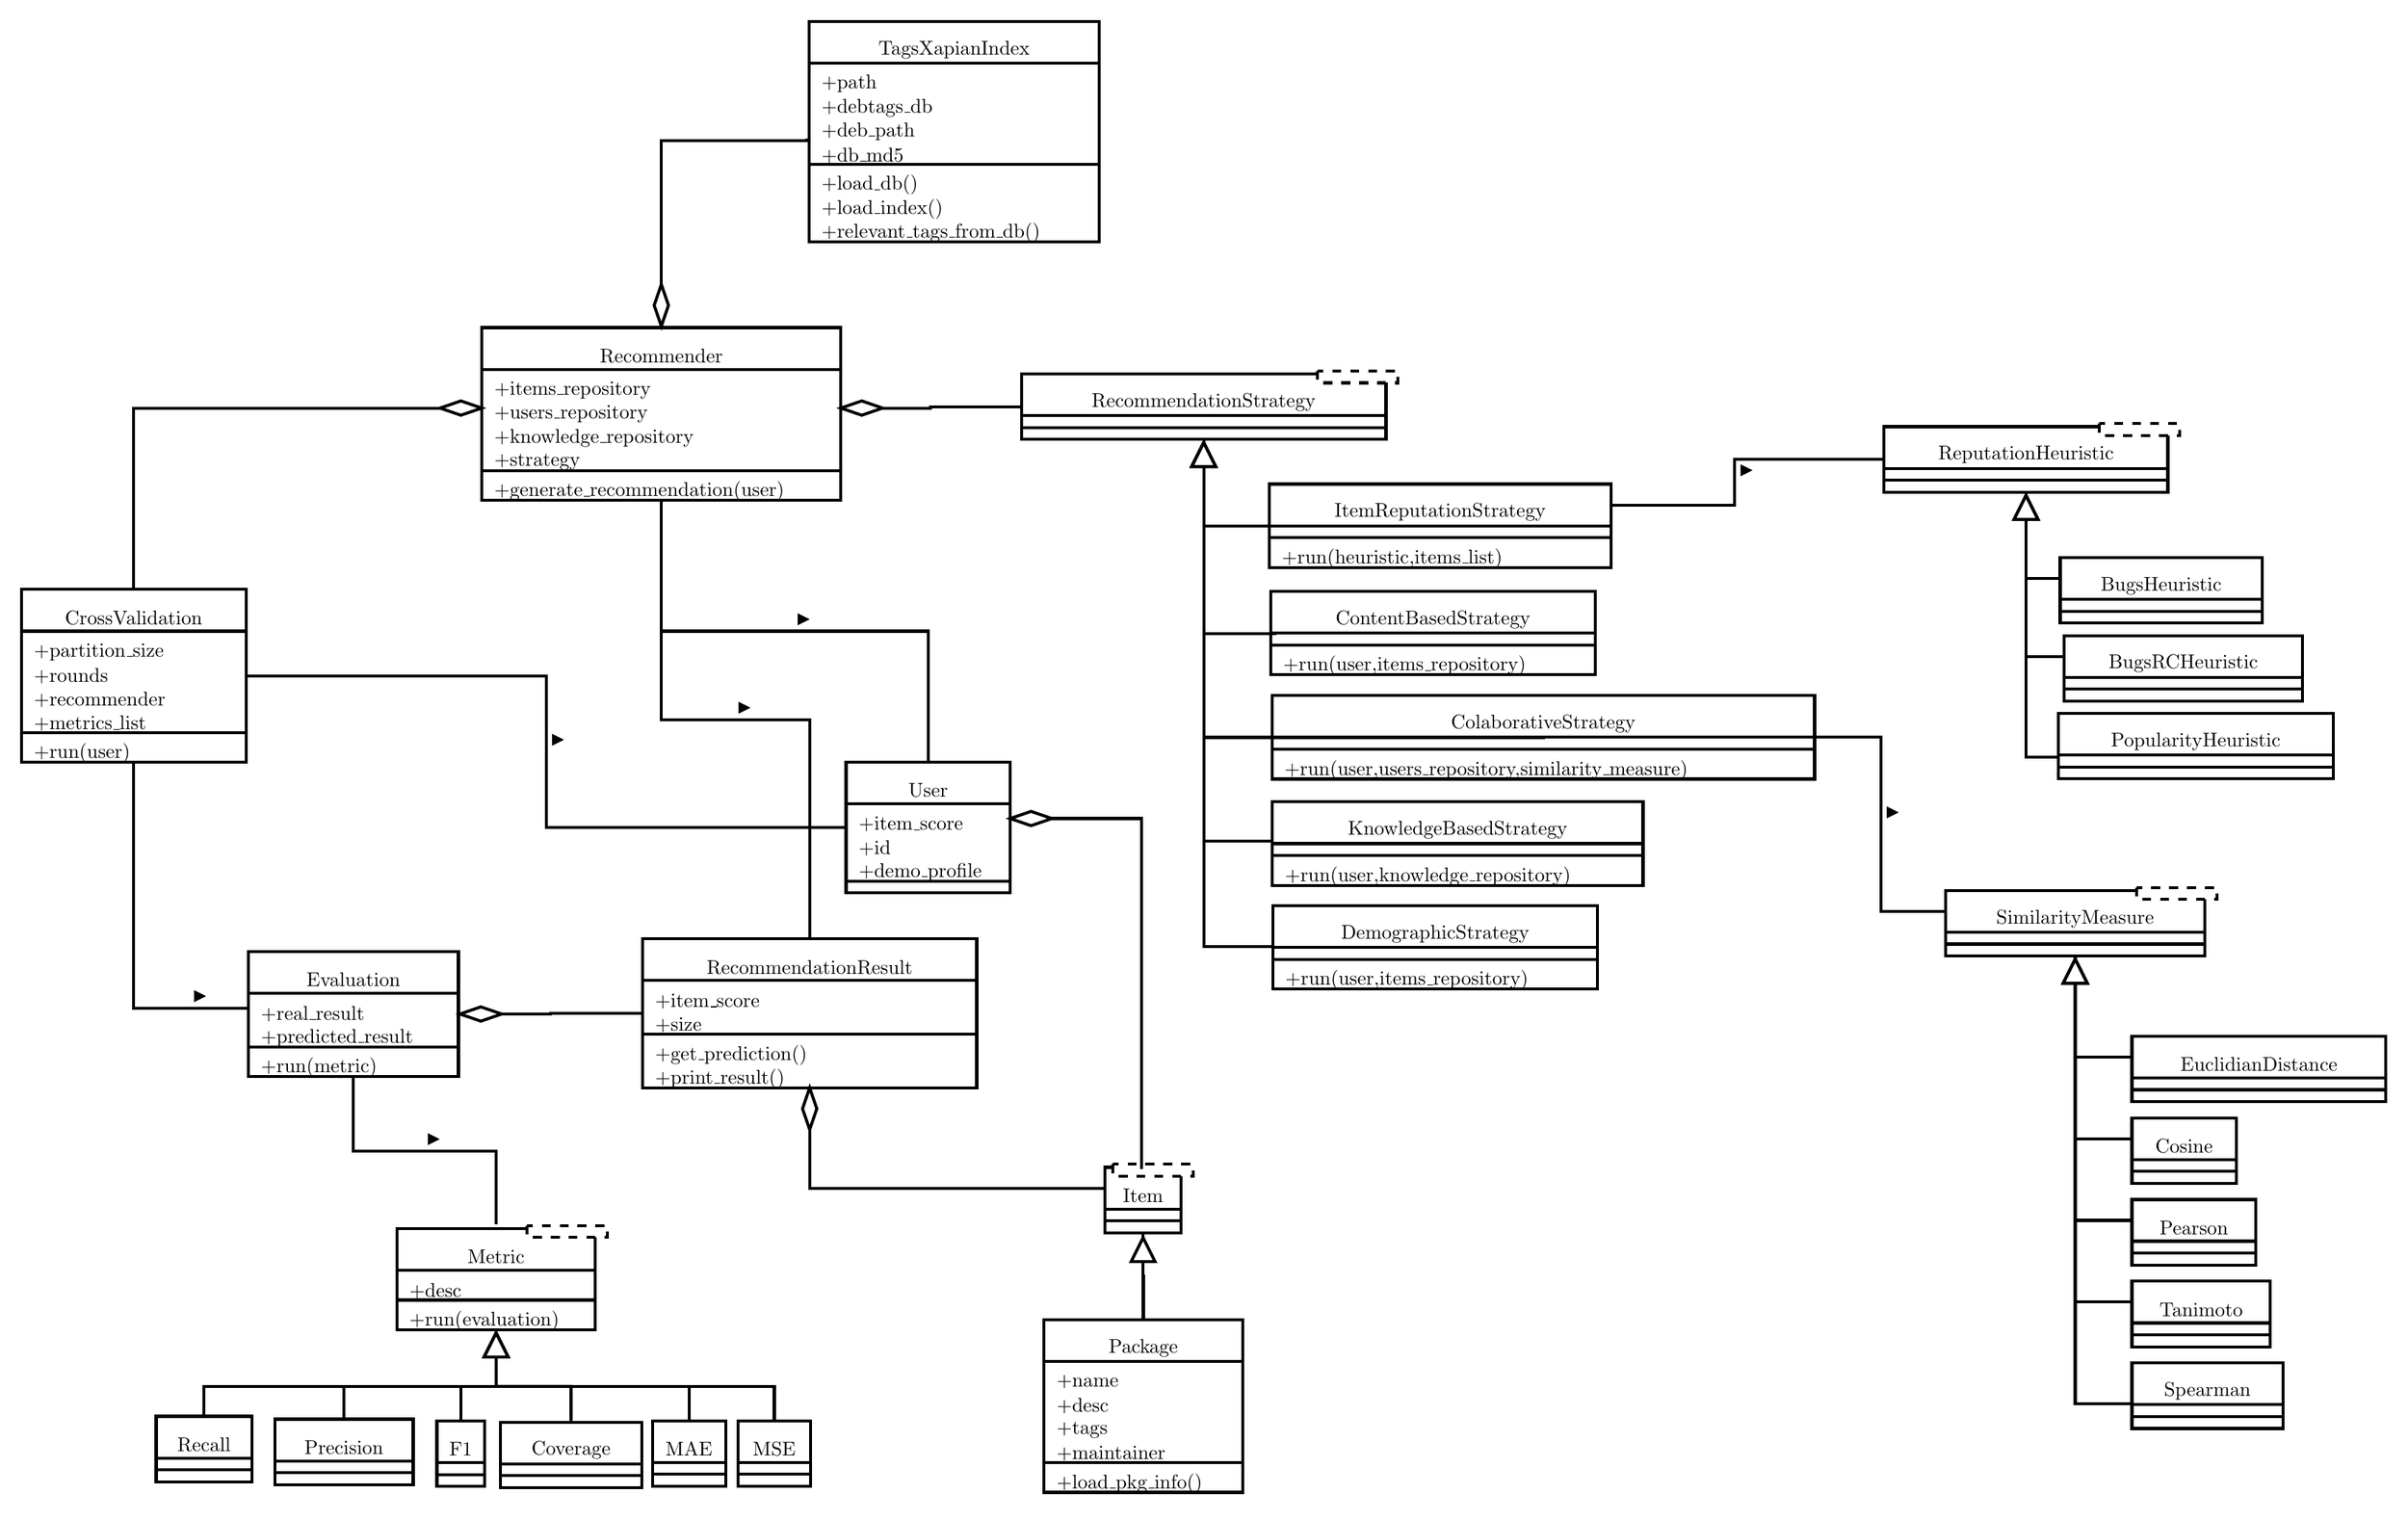
\begin{tikzpicture}
\pgftransformxscale{1.000000}
\pgftransformyscale{-1.000000}
\definecolor{dialinecolor}{rgb}{0.000000, 0.000000, 0.000000}
\pgfsetstrokecolor{dialinecolor}
\definecolor{dialinecolor}{rgb}{1.000000, 1.000000, 1.000000}
\pgfsetfillcolor{dialinecolor}
\pgfsetlinewidth{0.100000\du}
\pgfsetdash{}{0pt}
\definecolor{dialinecolor}{rgb}{1.000000, 1.000000, 1.000000}
\pgfsetfillcolor{dialinecolor}
\fill (10.296700\du,-25.289700\du)--(10.296700\du,-23.889700\du)--(22.346700\du,-23.889700\du)--(22.346700\du,-25.289700\du)--cycle;
\definecolor{dialinecolor}{rgb}{0.000000, 0.000000, 0.000000}
\pgfsetstrokecolor{dialinecolor}
\draw (10.296700\du,-25.289700\du)--(10.296700\du,-23.889700\du)--(22.346700\du,-23.889700\du)--(22.346700\du,-25.289700\du)--cycle;
% setfont left to latex
\definecolor{dialinecolor}{rgb}{0.000000, 0.000000, 0.000000}
\pgfsetstrokecolor{dialinecolor}
\node at (16.321700\du,-24.339700\du){Recommender};
\definecolor{dialinecolor}{rgb}{1.000000, 1.000000, 1.000000}
\pgfsetfillcolor{dialinecolor}
\fill (10.296700\du,-23.889700\du)--(10.296700\du,-20.489700\du)--(22.346700\du,-20.489700\du)--(22.346700\du,-23.889700\du)--cycle;
\definecolor{dialinecolor}{rgb}{0.000000, 0.000000, 0.000000}
\pgfsetstrokecolor{dialinecolor}
\draw (10.296700\du,-23.889700\du)--(10.296700\du,-20.489700\du)--(22.346700\du,-20.489700\du)--(22.346700\du,-23.889700\du)--cycle;
% setfont left to latex
\definecolor{dialinecolor}{rgb}{0.000000, 0.000000, 0.000000}
\pgfsetstrokecolor{dialinecolor}
\node[anchor=west] at (10.446700\du,-23.189700\du){+items\_repository};
% setfont left to latex
\definecolor{dialinecolor}{rgb}{0.000000, 0.000000, 0.000000}
\pgfsetstrokecolor{dialinecolor}
\node[anchor=west] at (10.446700\du,-22.389700\du){+users\_repository};
% setfont left to latex
\definecolor{dialinecolor}{rgb}{0.000000, 0.000000, 0.000000}
\pgfsetstrokecolor{dialinecolor}
\node[anchor=west] at (10.446700\du,-21.589700\du){+knowledge\_repository};
% setfont left to latex
\definecolor{dialinecolor}{rgb}{0.000000, 0.000000, 0.000000}
\pgfsetstrokecolor{dialinecolor}
\node[anchor=west] at (10.446700\du,-20.789700\du){+strategy};
\definecolor{dialinecolor}{rgb}{1.000000, 1.000000, 1.000000}
\pgfsetfillcolor{dialinecolor}
\fill (10.296700\du,-20.489700\du)--(10.296700\du,-19.489700\du)--(22.346700\du,-19.489700\du)--(22.346700\du,-20.489700\du)--cycle;
\definecolor{dialinecolor}{rgb}{0.000000, 0.000000, 0.000000}
\pgfsetstrokecolor{dialinecolor}
\draw (10.296700\du,-20.489700\du)--(10.296700\du,-19.489700\du)--(22.346700\du,-19.489700\du)--(22.346700\du,-20.489700\du)--cycle;
% setfont left to latex
\definecolor{dialinecolor}{rgb}{0.000000, 0.000000, 0.000000}
\pgfsetstrokecolor{dialinecolor}
\node[anchor=west] at (10.446700\du,-19.789700\du){+generate\_recommendation(user)};
\pgfsetlinewidth{0.100000\du}
\pgfsetdash{}{0pt}
\definecolor{dialinecolor}{rgb}{1.000000, 1.000000, 1.000000}
\pgfsetfillcolor{dialinecolor}
\fill (15.694400\du,-4.771430\du)--(15.694400\du,-3.371430\du)--(26.904400\du,-3.371430\du)--(26.904400\du,-4.771430\du)--cycle;
\definecolor{dialinecolor}{rgb}{0.000000, 0.000000, 0.000000}
\pgfsetstrokecolor{dialinecolor}
\draw (15.694400\du,-4.771430\du)--(15.694400\du,-3.371430\du)--(26.904400\du,-3.371430\du)--(26.904400\du,-4.771430\du)--cycle;
% setfont left to latex
\definecolor{dialinecolor}{rgb}{0.000000, 0.000000, 0.000000}
\pgfsetstrokecolor{dialinecolor}
\node at (21.299400\du,-3.821430\du){RecommendationResult};
\definecolor{dialinecolor}{rgb}{1.000000, 1.000000, 1.000000}
\pgfsetfillcolor{dialinecolor}
\fill (15.694400\du,-3.371430\du)--(15.694400\du,-1.571430\du)--(26.904400\du,-1.571430\du)--(26.904400\du,-3.371430\du)--cycle;
\definecolor{dialinecolor}{rgb}{0.000000, 0.000000, 0.000000}
\pgfsetstrokecolor{dialinecolor}
\draw (15.694400\du,-3.371430\du)--(15.694400\du,-1.571430\du)--(26.904400\du,-1.571430\du)--(26.904400\du,-3.371430\du)--cycle;
% setfont left to latex
\definecolor{dialinecolor}{rgb}{0.000000, 0.000000, 0.000000}
\pgfsetstrokecolor{dialinecolor}
\node[anchor=west] at (15.844400\du,-2.671430\du){+item\_score};
% setfont left to latex
\definecolor{dialinecolor}{rgb}{0.000000, 0.000000, 0.000000}
\pgfsetstrokecolor{dialinecolor}
\node[anchor=west] at (15.844400\du,-1.871430\du){+size};
\definecolor{dialinecolor}{rgb}{1.000000, 1.000000, 1.000000}
\pgfsetfillcolor{dialinecolor}
\fill (15.694400\du,-1.571430\du)--(15.694400\du,0.228570\du)--(26.904400\du,0.228570\du)--(26.904400\du,-1.571430\du)--cycle;
\definecolor{dialinecolor}{rgb}{0.000000, 0.000000, 0.000000}
\pgfsetstrokecolor{dialinecolor}
\draw (15.694400\du,-1.571430\du)--(15.694400\du,0.228570\du)--(26.904400\du,0.228570\du)--(26.904400\du,-1.571430\du)--cycle;
% setfont left to latex
\definecolor{dialinecolor}{rgb}{0.000000, 0.000000, 0.000000}
\pgfsetstrokecolor{dialinecolor}
\node[anchor=west] at (15.844400\du,-0.871430\du){+get\_prediction()};
% setfont left to latex
\definecolor{dialinecolor}{rgb}{0.000000, 0.000000, 0.000000}
\pgfsetstrokecolor{dialinecolor}
\node[anchor=west] at (15.844400\du,-0.071430\du){+print\_result()};
\pgfsetlinewidth{0.100000\du}
\pgfsetdash{}{0pt}
\definecolor{dialinecolor}{rgb}{1.000000, 1.000000, 1.000000}
\pgfsetfillcolor{dialinecolor}
\fill (-5.151470\du,-16.500000\du)--(-5.151470\du,-15.100000\du)--(2.388530\du,-15.100000\du)--(2.388530\du,-16.500000\du)--cycle;
\definecolor{dialinecolor}{rgb}{0.000000, 0.000000, 0.000000}
\pgfsetstrokecolor{dialinecolor}
\draw (-5.151470\du,-16.500000\du)--(-5.151470\du,-15.100000\du)--(2.388530\du,-15.100000\du)--(2.388530\du,-16.500000\du)--cycle;
% setfont left to latex
\definecolor{dialinecolor}{rgb}{0.000000, 0.000000, 0.000000}
\pgfsetstrokecolor{dialinecolor}
\node at (-1.381470\du,-15.550000\du){CrossValidation};
\definecolor{dialinecolor}{rgb}{1.000000, 1.000000, 1.000000}
\pgfsetfillcolor{dialinecolor}
\fill (-5.151470\du,-15.100000\du)--(-5.151470\du,-11.700000\du)--(2.388530\du,-11.700000\du)--(2.388530\du,-15.100000\du)--cycle;
\definecolor{dialinecolor}{rgb}{0.000000, 0.000000, 0.000000}
\pgfsetstrokecolor{dialinecolor}
\draw (-5.151470\du,-15.100000\du)--(-5.151470\du,-11.700000\du)--(2.388530\du,-11.700000\du)--(2.388530\du,-15.100000\du)--cycle;
% setfont left to latex
\definecolor{dialinecolor}{rgb}{0.000000, 0.000000, 0.000000}
\pgfsetstrokecolor{dialinecolor}
\node[anchor=west] at (-5.001470\du,-14.400000\du){+partition\_size};
% setfont left to latex
\definecolor{dialinecolor}{rgb}{0.000000, 0.000000, 0.000000}
\pgfsetstrokecolor{dialinecolor}
\node[anchor=west] at (-5.001470\du,-13.600000\du){+rounds};
% setfont left to latex
\definecolor{dialinecolor}{rgb}{0.000000, 0.000000, 0.000000}
\pgfsetstrokecolor{dialinecolor}
\node[anchor=west] at (-5.001470\du,-12.800000\du){+recommender};
% setfont left to latex
\definecolor{dialinecolor}{rgb}{0.000000, 0.000000, 0.000000}
\pgfsetstrokecolor{dialinecolor}
\node[anchor=west] at (-5.001470\du,-12.000000\du){+metrics\_list};
\definecolor{dialinecolor}{rgb}{1.000000, 1.000000, 1.000000}
\pgfsetfillcolor{dialinecolor}
\fill (-5.151470\du,-11.700000\du)--(-5.151470\du,-10.700000\du)--(2.388530\du,-10.700000\du)--(2.388530\du,-11.700000\du)--cycle;
\definecolor{dialinecolor}{rgb}{0.000000, 0.000000, 0.000000}
\pgfsetstrokecolor{dialinecolor}
\draw (-5.151470\du,-11.700000\du)--(-5.151470\du,-10.700000\du)--(2.388530\du,-10.700000\du)--(2.388530\du,-11.700000\du)--cycle;
% setfont left to latex
\definecolor{dialinecolor}{rgb}{0.000000, 0.000000, 0.000000}
\pgfsetstrokecolor{dialinecolor}
\node[anchor=west] at (-5.001470\du,-11.000000\du){+run(user)};
\pgfsetlinewidth{0.100000\du}
\pgfsetdash{}{0pt}
\definecolor{dialinecolor}{rgb}{1.000000, 1.000000, 1.000000}
\pgfsetfillcolor{dialinecolor}
\fill (22.522700\du,-10.712100\du)--(22.522700\du,-9.312100\du)--(28.027700\du,-9.312100\du)--(28.027700\du,-10.712100\du)--cycle;
\definecolor{dialinecolor}{rgb}{0.000000, 0.000000, 0.000000}
\pgfsetstrokecolor{dialinecolor}
\draw (22.522700\du,-10.712100\du)--(22.522700\du,-9.312100\du)--(28.027700\du,-9.312100\du)--(28.027700\du,-10.712100\du)--cycle;
% setfont left to latex
\definecolor{dialinecolor}{rgb}{0.000000, 0.000000, 0.000000}
\pgfsetstrokecolor{dialinecolor}
\node at (25.275200\du,-9.762100\du){User};
\definecolor{dialinecolor}{rgb}{1.000000, 1.000000, 1.000000}
\pgfsetfillcolor{dialinecolor}
\fill (22.522700\du,-9.312100\du)--(22.522700\du,-6.712100\du)--(28.027700\du,-6.712100\du)--(28.027700\du,-9.312100\du)--cycle;
\definecolor{dialinecolor}{rgb}{0.000000, 0.000000, 0.000000}
\pgfsetstrokecolor{dialinecolor}
\draw (22.522700\du,-9.312100\du)--(22.522700\du,-6.712100\du)--(28.027700\du,-6.712100\du)--(28.027700\du,-9.312100\du)--cycle;
% setfont left to latex
\definecolor{dialinecolor}{rgb}{0.000000, 0.000000, 0.000000}
\pgfsetstrokecolor{dialinecolor}
\node[anchor=west] at (22.672700\du,-8.612100\du){+item\_score};
% setfont left to latex
\definecolor{dialinecolor}{rgb}{0.000000, 0.000000, 0.000000}
\pgfsetstrokecolor{dialinecolor}
\node[anchor=west] at (22.672700\du,-7.812100\du){+id};
% setfont left to latex
\definecolor{dialinecolor}{rgb}{0.000000, 0.000000, 0.000000}
\pgfsetstrokecolor{dialinecolor}
\node[anchor=west] at (22.672700\du,-7.012100\du){+demo\_profile};
\definecolor{dialinecolor}{rgb}{1.000000, 1.000000, 1.000000}
\pgfsetfillcolor{dialinecolor}
\fill (22.522700\du,-6.712100\du)--(22.522700\du,-6.312100\du)--(28.027700\du,-6.312100\du)--(28.027700\du,-6.712100\du)--cycle;
\definecolor{dialinecolor}{rgb}{0.000000, 0.000000, 0.000000}
\pgfsetstrokecolor{dialinecolor}
\draw (22.522700\du,-6.712100\du)--(22.522700\du,-6.312100\du)--(28.027700\du,-6.312100\du)--(28.027700\du,-6.712100\du)--cycle;
\pgfsetlinewidth{0.100000\du}
\pgfsetdash{}{0pt}
\definecolor{dialinecolor}{rgb}{1.000000, 1.000000, 1.000000}
\pgfsetfillcolor{dialinecolor}
\fill (2.470000\du,-4.350000\du)--(2.470000\du,-2.950000\du)--(9.515000\du,-2.950000\du)--(9.515000\du,-4.350000\du)--cycle;
\definecolor{dialinecolor}{rgb}{0.000000, 0.000000, 0.000000}
\pgfsetstrokecolor{dialinecolor}
\draw (2.470000\du,-4.350000\du)--(2.470000\du,-2.950000\du)--(9.515000\du,-2.950000\du)--(9.515000\du,-4.350000\du)--cycle;
% setfont left to latex
\definecolor{dialinecolor}{rgb}{0.000000, 0.000000, 0.000000}
\pgfsetstrokecolor{dialinecolor}
\node at (5.992500\du,-3.400000\du){Evaluation};
\definecolor{dialinecolor}{rgb}{1.000000, 1.000000, 1.000000}
\pgfsetfillcolor{dialinecolor}
\fill (2.470000\du,-2.950000\du)--(2.470000\du,-1.150000\du)--(9.515000\du,-1.150000\du)--(9.515000\du,-2.950000\du)--cycle;
\definecolor{dialinecolor}{rgb}{0.000000, 0.000000, 0.000000}
\pgfsetstrokecolor{dialinecolor}
\draw (2.470000\du,-2.950000\du)--(2.470000\du,-1.150000\du)--(9.515000\du,-1.150000\du)--(9.515000\du,-2.950000\du)--cycle;
% setfont left to latex
\definecolor{dialinecolor}{rgb}{0.000000, 0.000000, 0.000000}
\pgfsetstrokecolor{dialinecolor}
\node[anchor=west] at (2.620000\du,-2.250000\du){+real\_result};
% setfont left to latex
\definecolor{dialinecolor}{rgb}{0.000000, 0.000000, 0.000000}
\pgfsetstrokecolor{dialinecolor}
\node[anchor=west] at (2.620000\du,-1.450000\du){+predicted\_result};
\definecolor{dialinecolor}{rgb}{1.000000, 1.000000, 1.000000}
\pgfsetfillcolor{dialinecolor}
\fill (2.470000\du,-1.150000\du)--(2.470000\du,-0.150000\du)--(9.515000\du,-0.150000\du)--(9.515000\du,-1.150000\du)--cycle;
\definecolor{dialinecolor}{rgb}{0.000000, 0.000000, 0.000000}
\pgfsetstrokecolor{dialinecolor}
\draw (2.470000\du,-1.150000\du)--(2.470000\du,-0.150000\du)--(9.515000\du,-0.150000\du)--(9.515000\du,-1.150000\du)--cycle;
% setfont left to latex
\definecolor{dialinecolor}{rgb}{0.000000, 0.000000, 0.000000}
\pgfsetstrokecolor{dialinecolor}
\node[anchor=west] at (2.620000\du,-0.450000\du){+run(metric)};
\pgfsetlinewidth{0.100000\du}
\pgfsetdash{}{0pt}
\pgfsetmiterjoin
\pgfsetbuttcap
{
\definecolor{dialinecolor}{rgb}{0.000000, 0.000000, 0.000000}
\pgfsetfillcolor{dialinecolor}
% was here!!!
\definecolor{dialinecolor}{rgb}{0.000000, 0.000000, 0.000000}
\pgfsetstrokecolor{dialinecolor}
\draw (9.565436\du,-2.250000\du)--(12.604745\du,-2.250000\du)--(12.604745\du,-2.271430\du)--(15.644055\du,-2.271430\du);
}
\definecolor{dialinecolor}{rgb}{0.000000, 0.000000, 0.000000}
\pgfsetstrokecolor{dialinecolor}
\draw (10.824015\du,-2.250000\du)--(12.604745\du,-2.250000\du)--(12.604745\du,-2.271430\du)--(15.644055\du,-2.271430\du);
\pgfsetdash{}{0pt}
\pgfsetmiterjoin
\pgfsetbuttcap
\definecolor{dialinecolor}{rgb}{1.000000, 1.000000, 1.000000}
\pgfsetfillcolor{dialinecolor}
\fill (9.565436\du,-2.250000\du)--(10.265436\du,-2.490000\du)--(10.965436\du,-2.250000\du)--(10.265436\du,-2.010000\du)--cycle;
\pgfsetlinewidth{0.100000\du}
\pgfsetdash{}{0pt}
\pgfsetmiterjoin
\pgfsetbuttcap
\definecolor{dialinecolor}{rgb}{0.000000, 0.000000, 0.000000}
\pgfsetstrokecolor{dialinecolor}
\draw (9.565436\du,-2.250000\du)--(10.265436\du,-2.490000\du)--(10.965436\du,-2.250000\du)--(10.265436\du,-2.010000\du)--cycle;
% setfont left to latex
\definecolor{dialinecolor}{rgb}{0.000000, 0.000000, 0.000000}
\pgfsetstrokecolor{dialinecolor}
\node[anchor=west] at (12.704745\du,-2.460715\du){};
\definecolor{dialinecolor}{rgb}{0.000000, 0.000000, 0.000000}
\pgfsetstrokecolor{dialinecolor}
\node[anchor=west] at (11.165436\du,-2.450000\du){};
\definecolor{dialinecolor}{rgb}{0.000000, 0.000000, 0.000000}
\pgfsetstrokecolor{dialinecolor}
\node[anchor=east] at (15.444055\du,-2.471430\du){};
\pgfsetlinewidth{0.100000\du}
\pgfsetdash{}{0pt}
\pgfsetmiterjoin
\pgfsetbuttcap
{
\definecolor{dialinecolor}{rgb}{0.000000, 0.000000, 0.000000}
\pgfsetfillcolor{dialinecolor}
% was here!!!
\definecolor{dialinecolor}{rgb}{0.000000, 0.000000, 0.000000}
\pgfsetstrokecolor{dialinecolor}
\draw (10.780000\du,4.799548\du)--(10.780000\du,2.349905\du)--(5.992500\du,2.349905\du)--(5.992500\du,-0.099738\du);
}
% setfont left to latex
\definecolor{dialinecolor}{rgb}{0.000000, 0.000000, 0.000000}
\pgfsetstrokecolor{dialinecolor}
\node at (8.386250\du,2.149905\du){};
\definecolor{dialinecolor}{rgb}{0.000000, 0.000000, 0.000000}
\pgfsetfillcolor{dialinecolor}
\fill (8.486250\du,2.149905\du)--(8.486250\du,1.749905\du)--(8.886250\du,1.949905\du)--cycle;
\definecolor{dialinecolor}{rgb}{0.000000, 0.000000, 0.000000}
\pgfsetstrokecolor{dialinecolor}
\node[anchor=west] at (10.980000\du,4.599548\du){};
\definecolor{dialinecolor}{rgb}{0.000000, 0.000000, 0.000000}
\pgfsetstrokecolor{dialinecolor}
\node[anchor=west] at (6.192500\du,0.500262\du){};
\pgfsetlinewidth{0.100000\du}
\pgfsetdash{}{0pt}
\definecolor{dialinecolor}{rgb}{1.000000, 1.000000, 1.000000}
\pgfsetfillcolor{dialinecolor}
\fill (29.165500\du,8.008580\du)--(29.165500\du,9.408580\du)--(35.825500\du,9.408580\du)--(35.825500\du,8.008580\du)--cycle;
\definecolor{dialinecolor}{rgb}{0.000000, 0.000000, 0.000000}
\pgfsetstrokecolor{dialinecolor}
\draw (29.165500\du,8.008580\du)--(29.165500\du,9.408580\du)--(35.825500\du,9.408580\du)--(35.825500\du,8.008580\du)--cycle;
% setfont left to latex
\definecolor{dialinecolor}{rgb}{0.000000, 0.000000, 0.000000}
\pgfsetstrokecolor{dialinecolor}
\node at (32.495500\du,8.958580\du){Package};
\definecolor{dialinecolor}{rgb}{1.000000, 1.000000, 1.000000}
\pgfsetfillcolor{dialinecolor}
\fill (29.165500\du,9.408580\du)--(29.165500\du,12.808580\du)--(35.825500\du,12.808580\du)--(35.825500\du,9.408580\du)--cycle;
\definecolor{dialinecolor}{rgb}{0.000000, 0.000000, 0.000000}
\pgfsetstrokecolor{dialinecolor}
\draw (29.165500\du,9.408580\du)--(29.165500\du,12.808580\du)--(35.825500\du,12.808580\du)--(35.825500\du,9.408580\du)--cycle;
% setfont left to latex
\definecolor{dialinecolor}{rgb}{0.000000, 0.000000, 0.000000}
\pgfsetstrokecolor{dialinecolor}
\node[anchor=west] at (29.315500\du,10.108580\du){+name};
% setfont left to latex
\definecolor{dialinecolor}{rgb}{0.000000, 0.000000, 0.000000}
\pgfsetstrokecolor{dialinecolor}
\node[anchor=west] at (29.315500\du,10.908580\du){+desc};
% setfont left to latex
\definecolor{dialinecolor}{rgb}{0.000000, 0.000000, 0.000000}
\pgfsetstrokecolor{dialinecolor}
\node[anchor=west] at (29.315500\du,11.708580\du){+tags};
% setfont left to latex
\definecolor{dialinecolor}{rgb}{0.000000, 0.000000, 0.000000}
\pgfsetstrokecolor{dialinecolor}
\node[anchor=west] at (29.315500\du,12.508580\du){+maintainer};
\definecolor{dialinecolor}{rgb}{1.000000, 1.000000, 1.000000}
\pgfsetfillcolor{dialinecolor}
\fill (29.165500\du,12.808580\du)--(29.165500\du,13.808580\du)--(35.825500\du,13.808580\du)--(35.825500\du,12.808580\du)--cycle;
\definecolor{dialinecolor}{rgb}{0.000000, 0.000000, 0.000000}
\pgfsetstrokecolor{dialinecolor}
\draw (29.165500\du,12.808580\du)--(29.165500\du,13.808580\du)--(35.825500\du,13.808580\du)--(35.825500\du,12.808580\du)--cycle;
% setfont left to latex
\definecolor{dialinecolor}{rgb}{0.000000, 0.000000, 0.000000}
\pgfsetstrokecolor{dialinecolor}
\node[anchor=west] at (29.315500\du,13.508580\du){+load\_pkg\_info()};
\pgfsetlinewidth{0.100000\du}
\pgfsetdash{}{0pt}
\pgfsetmiterjoin
\pgfsetbuttcap
{
\definecolor{dialinecolor}{rgb}{0.000000, 0.000000, 0.000000}
\pgfsetfillcolor{dialinecolor}
% was here!!!
\definecolor{dialinecolor}{rgb}{0.000000, 0.000000, 0.000000}
\pgfsetstrokecolor{dialinecolor}
\draw (22.472358\du,-8.512100\du)--(12.455677\du,-8.512100\du)--(12.455677\du,-13.600000\du)--(2.438996\du,-13.600000\du);
}
% setfont left to latex
\definecolor{dialinecolor}{rgb}{0.000000, 0.000000, 0.000000}
\pgfsetstrokecolor{dialinecolor}
\node[anchor=west] at (12.555677\du,-11.256050\du){};
\definecolor{dialinecolor}{rgb}{0.000000, 0.000000, 0.000000}
\pgfsetfillcolor{dialinecolor}
\fill (12.655677\du,-11.256050\du)--(12.655677\du,-11.656050\du)--(13.055677\du,-11.456050\du)--cycle;
\definecolor{dialinecolor}{rgb}{0.000000, 0.000000, 0.000000}
\pgfsetstrokecolor{dialinecolor}
\node[anchor=east] at (22.272358\du,-8.712100\du){};
\definecolor{dialinecolor}{rgb}{0.000000, 0.000000, 0.000000}
\pgfsetstrokecolor{dialinecolor}
\node[anchor=west] at (2.638996\du,-13.800000\du){};
\pgfsetlinewidth{0.100000\du}
\pgfsetdash{}{0pt}
\definecolor{dialinecolor}{rgb}{1.000000, 1.000000, 1.000000}
\pgfsetfillcolor{dialinecolor}
\fill (31.210100\du,2.895840\du)--(31.210100\du,4.295840\du)--(33.765100\du,4.295840\du)--(33.765100\du,2.895840\du)--cycle;
\definecolor{dialinecolor}{rgb}{0.000000, 0.000000, 0.000000}
\pgfsetstrokecolor{dialinecolor}
\draw (31.210100\du,2.895840\du)--(31.210100\du,4.295840\du)--(33.765100\du,4.295840\du)--(33.765100\du,2.895840\du)--cycle;
% setfont left to latex
\definecolor{dialinecolor}{rgb}{0.000000, 0.000000, 0.000000}
\pgfsetstrokecolor{dialinecolor}
\node at (32.487600\du,3.845840\du){Item};
\definecolor{dialinecolor}{rgb}{1.000000, 1.000000, 1.000000}
\pgfsetfillcolor{dialinecolor}
\fill (31.210100\du,4.295840\du)--(31.210100\du,4.695840\du)--(33.765100\du,4.695840\du)--(33.765100\du,4.295840\du)--cycle;
\definecolor{dialinecolor}{rgb}{0.000000, 0.000000, 0.000000}
\pgfsetstrokecolor{dialinecolor}
\draw (31.210100\du,4.295840\du)--(31.210100\du,4.695840\du)--(33.765100\du,4.695840\du)--(33.765100\du,4.295840\du)--cycle;
\definecolor{dialinecolor}{rgb}{1.000000, 1.000000, 1.000000}
\pgfsetfillcolor{dialinecolor}
\fill (31.210100\du,4.695840\du)--(31.210100\du,5.095840\du)--(33.765100\du,5.095840\du)--(33.765100\du,4.695840\du)--cycle;
\definecolor{dialinecolor}{rgb}{0.000000, 0.000000, 0.000000}
\pgfsetstrokecolor{dialinecolor}
\draw (31.210100\du,4.695840\du)--(31.210100\du,5.095840\du)--(33.765100\du,5.095840\du)--(33.765100\du,4.695840\du)--cycle;
\definecolor{dialinecolor}{rgb}{1.000000, 1.000000, 1.000000}
\pgfsetfillcolor{dialinecolor}
\fill (31.465100\du,2.795840\du)--(31.465100\du,3.195840\du)--(34.165100\du,3.195840\du)--(34.165100\du,2.795840\du)--cycle;
\pgfsetdash{{1.000000\du}{1.000000\du}}{0\du}
\pgfsetdash{{0.300000\du}{0.300000\du}}{0\du}
\definecolor{dialinecolor}{rgb}{0.000000, 0.000000, 0.000000}
\pgfsetstrokecolor{dialinecolor}
\draw (31.465100\du,2.795840\du)--(31.465100\du,3.195840\du)--(34.165100\du,3.195840\du)--(34.165100\du,2.795840\du)--cycle;
% setfont left to latex
\pgfsetlinewidth{0.100000\du}
\pgfsetdash{}{0pt}
\pgfsetmiterjoin
\pgfsetbuttcap
{
\definecolor{dialinecolor}{rgb}{0.000000, 0.000000, 0.000000}
\pgfsetfillcolor{dialinecolor}
% was here!!!
\definecolor{dialinecolor}{rgb}{0.000000, 0.000000, 0.000000}
\pgfsetstrokecolor{dialinecolor}
\draw (32.487600\du,5.146121\du)--(32.487600\du,6.552170\du)--(32.495500\du,6.552170\du)--(32.495500\du,7.958220\du);
}
\definecolor{dialinecolor}{rgb}{0.000000, 0.000000, 0.000000}
\pgfsetstrokecolor{dialinecolor}
\draw (32.487600\du,6.057924\du)--(32.487600\du,6.552170\du)--(32.495500\du,6.552170\du)--(32.495500\du,7.958220\du);
\pgfsetmiterjoin
\definecolor{dialinecolor}{rgb}{1.000000, 1.000000, 1.000000}
\pgfsetfillcolor{dialinecolor}
\fill (32.887600\du,6.057924\du)--(32.487600\du,5.257924\du)--(32.087600\du,6.057924\du)--cycle;
\pgfsetlinewidth{0.100000\du}
\pgfsetdash{}{0pt}
\pgfsetmiterjoin
\definecolor{dialinecolor}{rgb}{0.000000, 0.000000, 0.000000}
\pgfsetstrokecolor{dialinecolor}
\draw (32.887600\du,6.057924\du)--(32.487600\du,5.257924\du)--(32.087600\du,6.057924\du)--cycle;
% setfont left to latex
\pgfsetlinewidth{0.100000\du}
\pgfsetdash{}{0pt}
\definecolor{dialinecolor}{rgb}{1.000000, 1.000000, 1.000000}
\pgfsetfillcolor{dialinecolor}
\fill (7.450000\du,4.950000\du)--(7.450000\du,6.350000\du)--(14.110000\du,6.350000\du)--(14.110000\du,4.950000\du)--cycle;
\definecolor{dialinecolor}{rgb}{0.000000, 0.000000, 0.000000}
\pgfsetstrokecolor{dialinecolor}
\draw (7.450000\du,4.950000\du)--(7.450000\du,6.350000\du)--(14.110000\du,6.350000\du)--(14.110000\du,4.950000\du)--cycle;
% setfont left to latex
\definecolor{dialinecolor}{rgb}{0.000000, 0.000000, 0.000000}
\pgfsetstrokecolor{dialinecolor}
\node at (10.780000\du,5.900000\du){Metric};
\definecolor{dialinecolor}{rgb}{1.000000, 1.000000, 1.000000}
\pgfsetfillcolor{dialinecolor}
\fill (7.450000\du,6.350000\du)--(7.450000\du,7.350000\du)--(14.110000\du,7.350000\du)--(14.110000\du,6.350000\du)--cycle;
\definecolor{dialinecolor}{rgb}{0.000000, 0.000000, 0.000000}
\pgfsetstrokecolor{dialinecolor}
\draw (7.450000\du,6.350000\du)--(7.450000\du,7.350000\du)--(14.110000\du,7.350000\du)--(14.110000\du,6.350000\du)--cycle;
% setfont left to latex
\definecolor{dialinecolor}{rgb}{0.000000, 0.000000, 0.000000}
\pgfsetstrokecolor{dialinecolor}
\node[anchor=west] at (7.600000\du,7.050000\du){+desc};
\definecolor{dialinecolor}{rgb}{1.000000, 1.000000, 1.000000}
\pgfsetfillcolor{dialinecolor}
\fill (7.450000\du,7.350000\du)--(7.450000\du,8.350000\du)--(14.110000\du,8.350000\du)--(14.110000\du,7.350000\du)--cycle;
\definecolor{dialinecolor}{rgb}{0.000000, 0.000000, 0.000000}
\pgfsetstrokecolor{dialinecolor}
\draw (7.450000\du,7.350000\du)--(7.450000\du,8.350000\du)--(14.110000\du,8.350000\du)--(14.110000\du,7.350000\du)--cycle;
% setfont left to latex
\definecolor{dialinecolor}{rgb}{0.000000, 0.000000, 0.000000}
\pgfsetstrokecolor{dialinecolor}
\node[anchor=west] at (7.600000\du,8.050000\du){+run(evaluation)};
\definecolor{dialinecolor}{rgb}{1.000000, 1.000000, 1.000000}
\pgfsetfillcolor{dialinecolor}
\fill (11.810000\du,4.850000\du)--(11.810000\du,5.250000\du)--(14.510000\du,5.250000\du)--(14.510000\du,4.850000\du)--cycle;
\pgfsetdash{{0.300000\du}{0.300000\du}}{0\du}
\pgfsetdash{{0.300000\du}{0.300000\du}}{0\du}
\definecolor{dialinecolor}{rgb}{0.000000, 0.000000, 0.000000}
\pgfsetstrokecolor{dialinecolor}
\draw (11.810000\du,4.850000\du)--(11.810000\du,5.250000\du)--(14.510000\du,5.250000\du)--(14.510000\du,4.850000\du)--cycle;
% setfont left to latex
\pgfsetlinewidth{0.100000\du}
\pgfsetdash{}{0pt}
\definecolor{dialinecolor}{rgb}{1.000000, 1.000000, 1.000000}
\pgfsetfillcolor{dialinecolor}
\fill (3.350000\du,11.350000\du)--(3.350000\du,12.750000\du)--(7.995000\du,12.750000\du)--(7.995000\du,11.350000\du)--cycle;
\definecolor{dialinecolor}{rgb}{0.000000, 0.000000, 0.000000}
\pgfsetstrokecolor{dialinecolor}
\draw (3.350000\du,11.350000\du)--(3.350000\du,12.750000\du)--(7.995000\du,12.750000\du)--(7.995000\du,11.350000\du)--cycle;
% setfont left to latex
\definecolor{dialinecolor}{rgb}{0.000000, 0.000000, 0.000000}
\pgfsetstrokecolor{dialinecolor}
\node at (5.672500\du,12.300000\du){Precision};
\definecolor{dialinecolor}{rgb}{1.000000, 1.000000, 1.000000}
\pgfsetfillcolor{dialinecolor}
\fill (3.350000\du,12.750000\du)--(3.350000\du,13.150000\du)--(7.995000\du,13.150000\du)--(7.995000\du,12.750000\du)--cycle;
\definecolor{dialinecolor}{rgb}{0.000000, 0.000000, 0.000000}
\pgfsetstrokecolor{dialinecolor}
\draw (3.350000\du,12.750000\du)--(3.350000\du,13.150000\du)--(7.995000\du,13.150000\du)--(7.995000\du,12.750000\du)--cycle;
\definecolor{dialinecolor}{rgb}{1.000000, 1.000000, 1.000000}
\pgfsetfillcolor{dialinecolor}
\fill (3.350000\du,13.150000\du)--(3.350000\du,13.550000\du)--(7.995000\du,13.550000\du)--(7.995000\du,13.150000\du)--cycle;
\definecolor{dialinecolor}{rgb}{0.000000, 0.000000, 0.000000}
\pgfsetstrokecolor{dialinecolor}
\draw (3.350000\du,13.150000\du)--(3.350000\du,13.550000\du)--(7.995000\du,13.550000\du)--(7.995000\du,13.150000\du)--cycle;
\pgfsetlinewidth{0.100000\du}
\pgfsetdash{}{0pt}
\definecolor{dialinecolor}{rgb}{1.000000, 1.000000, 1.000000}
\pgfsetfillcolor{dialinecolor}
\fill (-0.630000\du,11.255000\du)--(-0.630000\du,12.655000\du)--(2.592500\du,12.655000\du)--(2.592500\du,11.255000\du)--cycle;
\definecolor{dialinecolor}{rgb}{0.000000, 0.000000, 0.000000}
\pgfsetstrokecolor{dialinecolor}
\draw (-0.630000\du,11.255000\du)--(-0.630000\du,12.655000\du)--(2.592500\du,12.655000\du)--(2.592500\du,11.255000\du)--cycle;
% setfont left to latex
\definecolor{dialinecolor}{rgb}{0.000000, 0.000000, 0.000000}
\pgfsetstrokecolor{dialinecolor}
\node at (0.981250\du,12.205000\du){Recall};
\definecolor{dialinecolor}{rgb}{1.000000, 1.000000, 1.000000}
\pgfsetfillcolor{dialinecolor}
\fill (-0.630000\du,12.655000\du)--(-0.630000\du,13.055000\du)--(2.592500\du,13.055000\du)--(2.592500\du,12.655000\du)--cycle;
\definecolor{dialinecolor}{rgb}{0.000000, 0.000000, 0.000000}
\pgfsetstrokecolor{dialinecolor}
\draw (-0.630000\du,12.655000\du)--(-0.630000\du,13.055000\du)--(2.592500\du,13.055000\du)--(2.592500\du,12.655000\du)--cycle;
\definecolor{dialinecolor}{rgb}{1.000000, 1.000000, 1.000000}
\pgfsetfillcolor{dialinecolor}
\fill (-0.630000\du,13.055000\du)--(-0.630000\du,13.455000\du)--(2.592500\du,13.455000\du)--(2.592500\du,13.055000\du)--cycle;
\definecolor{dialinecolor}{rgb}{0.000000, 0.000000, 0.000000}
\pgfsetstrokecolor{dialinecolor}
\draw (-0.630000\du,13.055000\du)--(-0.630000\du,13.455000\du)--(2.592500\du,13.455000\du)--(2.592500\du,13.055000\du)--cycle;
\pgfsetlinewidth{0.100000\du}
\pgfsetdash{}{0pt}
\definecolor{dialinecolor}{rgb}{1.000000, 1.000000, 1.000000}
\pgfsetfillcolor{dialinecolor}
\fill (8.790000\du,11.410000\du)--(8.790000\du,12.810000\du)--(10.395000\du,12.810000\du)--(10.395000\du,11.410000\du)--cycle;
\definecolor{dialinecolor}{rgb}{0.000000, 0.000000, 0.000000}
\pgfsetstrokecolor{dialinecolor}
\draw (8.790000\du,11.410000\du)--(8.790000\du,12.810000\du)--(10.395000\du,12.810000\du)--(10.395000\du,11.410000\du)--cycle;
% setfont left to latex
\definecolor{dialinecolor}{rgb}{0.000000, 0.000000, 0.000000}
\pgfsetstrokecolor{dialinecolor}
\node at (9.592500\du,12.360000\du){F1};
\definecolor{dialinecolor}{rgb}{1.000000, 1.000000, 1.000000}
\pgfsetfillcolor{dialinecolor}
\fill (8.790000\du,12.810000\du)--(8.790000\du,13.210000\du)--(10.395000\du,13.210000\du)--(10.395000\du,12.810000\du)--cycle;
\definecolor{dialinecolor}{rgb}{0.000000, 0.000000, 0.000000}
\pgfsetstrokecolor{dialinecolor}
\draw (8.790000\du,12.810000\du)--(8.790000\du,13.210000\du)--(10.395000\du,13.210000\du)--(10.395000\du,12.810000\du)--cycle;
\definecolor{dialinecolor}{rgb}{1.000000, 1.000000, 1.000000}
\pgfsetfillcolor{dialinecolor}
\fill (8.790000\du,13.210000\du)--(8.790000\du,13.610000\du)--(10.395000\du,13.610000\du)--(10.395000\du,13.210000\du)--cycle;
\definecolor{dialinecolor}{rgb}{0.000000, 0.000000, 0.000000}
\pgfsetstrokecolor{dialinecolor}
\draw (8.790000\du,13.210000\du)--(8.790000\du,13.610000\du)--(10.395000\du,13.610000\du)--(10.395000\du,13.210000\du)--cycle;
\pgfsetlinewidth{0.100000\du}
\pgfsetdash{}{0pt}
\definecolor{dialinecolor}{rgb}{1.000000, 1.000000, 1.000000}
\pgfsetfillcolor{dialinecolor}
\fill (10.915000\du,11.450000\du)--(10.915000\du,12.850000\du)--(15.667500\du,12.850000\du)--(15.667500\du,11.450000\du)--cycle;
\definecolor{dialinecolor}{rgb}{0.000000, 0.000000, 0.000000}
\pgfsetstrokecolor{dialinecolor}
\draw (10.915000\du,11.450000\du)--(10.915000\du,12.850000\du)--(15.667500\du,12.850000\du)--(15.667500\du,11.450000\du)--cycle;
% setfont left to latex
\definecolor{dialinecolor}{rgb}{0.000000, 0.000000, 0.000000}
\pgfsetstrokecolor{dialinecolor}
\node at (13.291250\du,12.400000\du){Coverage};
\definecolor{dialinecolor}{rgb}{1.000000, 1.000000, 1.000000}
\pgfsetfillcolor{dialinecolor}
\fill (10.915000\du,12.850000\du)--(10.915000\du,13.250000\du)--(15.667500\du,13.250000\du)--(15.667500\du,12.850000\du)--cycle;
\definecolor{dialinecolor}{rgb}{0.000000, 0.000000, 0.000000}
\pgfsetstrokecolor{dialinecolor}
\draw (10.915000\du,12.850000\du)--(10.915000\du,13.250000\du)--(15.667500\du,13.250000\du)--(15.667500\du,12.850000\du)--cycle;
\definecolor{dialinecolor}{rgb}{1.000000, 1.000000, 1.000000}
\pgfsetfillcolor{dialinecolor}
\fill (10.915000\du,13.250000\du)--(10.915000\du,13.650000\du)--(15.667500\du,13.650000\du)--(15.667500\du,13.250000\du)--cycle;
\definecolor{dialinecolor}{rgb}{0.000000, 0.000000, 0.000000}
\pgfsetstrokecolor{dialinecolor}
\draw (10.915000\du,13.250000\du)--(10.915000\du,13.650000\du)--(15.667500\du,13.650000\du)--(15.667500\du,13.250000\du)--cycle;
\pgfsetlinewidth{0.100000\du}
\pgfsetdash{}{0pt}
\definecolor{dialinecolor}{rgb}{1.000000, 1.000000, 1.000000}
\pgfsetfillcolor{dialinecolor}
\fill (16.020000\du,11.400000\du)--(16.020000\du,12.800000\du)--(18.482500\du,12.800000\du)--(18.482500\du,11.400000\du)--cycle;
\definecolor{dialinecolor}{rgb}{0.000000, 0.000000, 0.000000}
\pgfsetstrokecolor{dialinecolor}
\draw (16.020000\du,11.400000\du)--(16.020000\du,12.800000\du)--(18.482500\du,12.800000\du)--(18.482500\du,11.400000\du)--cycle;
% setfont left to latex
\definecolor{dialinecolor}{rgb}{0.000000, 0.000000, 0.000000}
\pgfsetstrokecolor{dialinecolor}
\node at (17.251250\du,12.350000\du){MAE};
\definecolor{dialinecolor}{rgb}{1.000000, 1.000000, 1.000000}
\pgfsetfillcolor{dialinecolor}
\fill (16.020000\du,12.800000\du)--(16.020000\du,13.200000\du)--(18.482500\du,13.200000\du)--(18.482500\du,12.800000\du)--cycle;
\definecolor{dialinecolor}{rgb}{0.000000, 0.000000, 0.000000}
\pgfsetstrokecolor{dialinecolor}
\draw (16.020000\du,12.800000\du)--(16.020000\du,13.200000\du)--(18.482500\du,13.200000\du)--(18.482500\du,12.800000\du)--cycle;
\definecolor{dialinecolor}{rgb}{1.000000, 1.000000, 1.000000}
\pgfsetfillcolor{dialinecolor}
\fill (16.020000\du,13.200000\du)--(16.020000\du,13.600000\du)--(18.482500\du,13.600000\du)--(18.482500\du,13.200000\du)--cycle;
\definecolor{dialinecolor}{rgb}{0.000000, 0.000000, 0.000000}
\pgfsetstrokecolor{dialinecolor}
\draw (16.020000\du,13.200000\du)--(16.020000\du,13.600000\du)--(18.482500\du,13.600000\du)--(18.482500\du,13.200000\du)--cycle;
\pgfsetlinewidth{0.100000\du}
\pgfsetdash{}{0pt}
\definecolor{dialinecolor}{rgb}{1.000000, 1.000000, 1.000000}
\pgfsetfillcolor{dialinecolor}
\fill (18.905000\du,11.400000\du)--(18.905000\du,12.800000\du)--(21.322500\du,12.800000\du)--(21.322500\du,11.400000\du)--cycle;
\definecolor{dialinecolor}{rgb}{0.000000, 0.000000, 0.000000}
\pgfsetstrokecolor{dialinecolor}
\draw (18.905000\du,11.400000\du)--(18.905000\du,12.800000\du)--(21.322500\du,12.800000\du)--(21.322500\du,11.400000\du)--cycle;
% setfont left to latex
\definecolor{dialinecolor}{rgb}{0.000000, 0.000000, 0.000000}
\pgfsetstrokecolor{dialinecolor}
\node at (20.113750\du,12.350000\du){MSE};
\definecolor{dialinecolor}{rgb}{1.000000, 1.000000, 1.000000}
\pgfsetfillcolor{dialinecolor}
\fill (18.905000\du,12.800000\du)--(18.905000\du,13.200000\du)--(21.322500\du,13.200000\du)--(21.322500\du,12.800000\du)--cycle;
\definecolor{dialinecolor}{rgb}{0.000000, 0.000000, 0.000000}
\pgfsetstrokecolor{dialinecolor}
\draw (18.905000\du,12.800000\du)--(18.905000\du,13.200000\du)--(21.322500\du,13.200000\du)--(21.322500\du,12.800000\du)--cycle;
\definecolor{dialinecolor}{rgb}{1.000000, 1.000000, 1.000000}
\pgfsetfillcolor{dialinecolor}
\fill (18.905000\du,13.200000\du)--(18.905000\du,13.600000\du)--(21.322500\du,13.600000\du)--(21.322500\du,13.200000\du)--cycle;
\definecolor{dialinecolor}{rgb}{0.000000, 0.000000, 0.000000}
\pgfsetstrokecolor{dialinecolor}
\draw (18.905000\du,13.200000\du)--(18.905000\du,13.600000\du)--(21.322500\du,13.600000\du)--(21.322500\du,13.200000\du)--cycle;
\pgfsetlinewidth{0.100000\du}
\pgfsetdash{}{0pt}
\pgfsetmiterjoin
\pgfsetbuttcap
{
\definecolor{dialinecolor}{rgb}{0.000000, 0.000000, 0.000000}
\pgfsetfillcolor{dialinecolor}
% was here!!!
\definecolor{dialinecolor}{rgb}{0.000000, 0.000000, 0.000000}
\pgfsetstrokecolor{dialinecolor}
\draw (10.780000\du,8.350000\du)--(10.780000\du,10.250000\du)--(5.672500\du,10.250000\du)--(5.672500\du,11.350000\du);
}
\definecolor{dialinecolor}{rgb}{0.000000, 0.000000, 0.000000}
\pgfsetstrokecolor{dialinecolor}
\draw (10.780000\du,9.261803\du)--(10.780000\du,10.250000\du)--(5.672500\du,10.250000\du)--(5.672500\du,11.350000\du);
\pgfsetmiterjoin
\definecolor{dialinecolor}{rgb}{1.000000, 1.000000, 1.000000}
\pgfsetfillcolor{dialinecolor}
\fill (11.180000\du,9.261803\du)--(10.780000\du,8.461803\du)--(10.380000\du,9.261803\du)--cycle;
\pgfsetlinewidth{0.100000\du}
\pgfsetdash{}{0pt}
\pgfsetmiterjoin
\definecolor{dialinecolor}{rgb}{0.000000, 0.000000, 0.000000}
\pgfsetstrokecolor{dialinecolor}
\draw (11.180000\du,9.261803\du)--(10.780000\du,8.461803\du)--(10.380000\du,9.261803\du)--cycle;
% setfont left to latex
\pgfsetlinewidth{0.100000\du}
\pgfsetdash{}{0pt}
\pgfsetmiterjoin
\pgfsetbuttcap
{
\definecolor{dialinecolor}{rgb}{0.000000, 0.000000, 0.000000}
\pgfsetfillcolor{dialinecolor}
% was here!!!
\definecolor{dialinecolor}{rgb}{0.000000, 0.000000, 0.000000}
\pgfsetstrokecolor{dialinecolor}
\draw (10.780000\du,8.350000\du)--(10.780000\du,10.250000\du)--(9.592500\du,10.250000\du)--(9.592500\du,11.410000\du);
}
\definecolor{dialinecolor}{rgb}{0.000000, 0.000000, 0.000000}
\pgfsetstrokecolor{dialinecolor}
\draw (10.780000\du,9.261803\du)--(10.780000\du,10.250000\du)--(9.592500\du,10.250000\du)--(9.592500\du,11.410000\du);
\pgfsetmiterjoin
\definecolor{dialinecolor}{rgb}{1.000000, 1.000000, 1.000000}
\pgfsetfillcolor{dialinecolor}
\fill (11.180000\du,9.261803\du)--(10.780000\du,8.461803\du)--(10.380000\du,9.261803\du)--cycle;
\pgfsetlinewidth{0.100000\du}
\pgfsetdash{}{0pt}
\pgfsetmiterjoin
\definecolor{dialinecolor}{rgb}{0.000000, 0.000000, 0.000000}
\pgfsetstrokecolor{dialinecolor}
\draw (11.180000\du,9.261803\du)--(10.780000\du,8.461803\du)--(10.380000\du,9.261803\du)--cycle;
% setfont left to latex
\pgfsetlinewidth{0.100000\du}
\pgfsetdash{}{0pt}
\pgfsetmiterjoin
\pgfsetbuttcap
{
\definecolor{dialinecolor}{rgb}{0.000000, 0.000000, 0.000000}
\pgfsetfillcolor{dialinecolor}
% was here!!!
\definecolor{dialinecolor}{rgb}{0.000000, 0.000000, 0.000000}
\pgfsetstrokecolor{dialinecolor}
\draw (10.780000\du,8.350000\du)--(10.780000\du,10.250000\du)--(0.981250\du,10.250000\du)--(0.981250\du,11.255000\du);
}
\definecolor{dialinecolor}{rgb}{0.000000, 0.000000, 0.000000}
\pgfsetstrokecolor{dialinecolor}
\draw (10.780000\du,9.261803\du)--(10.780000\du,10.250000\du)--(0.981250\du,10.250000\du)--(0.981250\du,11.255000\du);
\pgfsetmiterjoin
\definecolor{dialinecolor}{rgb}{1.000000, 1.000000, 1.000000}
\pgfsetfillcolor{dialinecolor}
\fill (11.180000\du,9.261803\du)--(10.780000\du,8.461803\du)--(10.380000\du,9.261803\du)--cycle;
\pgfsetlinewidth{0.100000\du}
\pgfsetdash{}{0pt}
\pgfsetmiterjoin
\definecolor{dialinecolor}{rgb}{0.000000, 0.000000, 0.000000}
\pgfsetstrokecolor{dialinecolor}
\draw (11.180000\du,9.261803\du)--(10.780000\du,8.461803\du)--(10.380000\du,9.261803\du)--cycle;
% setfont left to latex
\pgfsetlinewidth{0.100000\du}
\pgfsetdash{}{0pt}
\pgfsetmiterjoin
\pgfsetbuttcap
{
\definecolor{dialinecolor}{rgb}{0.000000, 0.000000, 0.000000}
\pgfsetfillcolor{dialinecolor}
% was here!!!
\definecolor{dialinecolor}{rgb}{0.000000, 0.000000, 0.000000}
\pgfsetstrokecolor{dialinecolor}
\draw (10.780000\du,8.350000\du)--(10.780000\du,10.250000\du)--(13.291225\du,10.250000\du)--(13.291237\du,11.399719\du);
}
\definecolor{dialinecolor}{rgb}{0.000000, 0.000000, 0.000000}
\pgfsetstrokecolor{dialinecolor}
\draw (10.780000\du,9.261803\du)--(10.780000\du,10.250000\du)--(13.291225\du,10.250000\du)--(13.291237\du,11.399719\du);
\pgfsetmiterjoin
\definecolor{dialinecolor}{rgb}{1.000000, 1.000000, 1.000000}
\pgfsetfillcolor{dialinecolor}
\fill (11.180000\du,9.261803\du)--(10.780000\du,8.461803\du)--(10.380000\du,9.261803\du)--cycle;
\pgfsetlinewidth{0.100000\du}
\pgfsetdash{}{0pt}
\pgfsetmiterjoin
\definecolor{dialinecolor}{rgb}{0.000000, 0.000000, 0.000000}
\pgfsetstrokecolor{dialinecolor}
\draw (11.180000\du,9.261803\du)--(10.780000\du,8.461803\du)--(10.380000\du,9.261803\du)--cycle;
% setfont left to latex
\pgfsetlinewidth{0.100000\du}
\pgfsetdash{}{0pt}
\pgfsetmiterjoin
\pgfsetbuttcap
{
\definecolor{dialinecolor}{rgb}{0.000000, 0.000000, 0.000000}
\pgfsetfillcolor{dialinecolor}
% was here!!!
\definecolor{dialinecolor}{rgb}{0.000000, 0.000000, 0.000000}
\pgfsetstrokecolor{dialinecolor}
\draw (10.780000\du,8.350000\du)--(10.780000\du,10.250000\du)--(17.251200\du,10.250000\du)--(17.251200\du,11.400000\du);
}
\definecolor{dialinecolor}{rgb}{0.000000, 0.000000, 0.000000}
\pgfsetstrokecolor{dialinecolor}
\draw (10.780000\du,9.261803\du)--(10.780000\du,10.250000\du)--(17.251200\du,10.250000\du)--(17.251200\du,11.400000\du);
\pgfsetmiterjoin
\definecolor{dialinecolor}{rgb}{1.000000, 1.000000, 1.000000}
\pgfsetfillcolor{dialinecolor}
\fill (11.180000\du,9.261803\du)--(10.780000\du,8.461803\du)--(10.380000\du,9.261803\du)--cycle;
\pgfsetlinewidth{0.100000\du}
\pgfsetdash{}{0pt}
\pgfsetmiterjoin
\definecolor{dialinecolor}{rgb}{0.000000, 0.000000, 0.000000}
\pgfsetstrokecolor{dialinecolor}
\draw (11.180000\du,9.261803\du)--(10.780000\du,8.461803\du)--(10.380000\du,9.261803\du)--cycle;
% setfont left to latex
\pgfsetlinewidth{0.100000\du}
\pgfsetdash{}{0pt}
\pgfsetmiterjoin
\pgfsetbuttcap
{
\definecolor{dialinecolor}{rgb}{0.000000, 0.000000, 0.000000}
\pgfsetfillcolor{dialinecolor}
% was here!!!
\definecolor{dialinecolor}{rgb}{0.000000, 0.000000, 0.000000}
\pgfsetstrokecolor{dialinecolor}
\draw (10.780000\du,8.350000\du)--(10.780000\du,10.250000\du)--(20.113700\du,10.250000\du)--(20.113700\du,11.400000\du);
}
\definecolor{dialinecolor}{rgb}{0.000000, 0.000000, 0.000000}
\pgfsetstrokecolor{dialinecolor}
\draw (10.780000\du,9.261803\du)--(10.780000\du,10.250000\du)--(20.113700\du,10.250000\du)--(20.113700\du,11.400000\du);
\pgfsetmiterjoin
\definecolor{dialinecolor}{rgb}{1.000000, 1.000000, 1.000000}
\pgfsetfillcolor{dialinecolor}
\fill (11.180000\du,9.261803\du)--(10.780000\du,8.461803\du)--(10.380000\du,9.261803\du)--cycle;
\pgfsetlinewidth{0.100000\du}
\pgfsetdash{}{0pt}
\pgfsetmiterjoin
\definecolor{dialinecolor}{rgb}{0.000000, 0.000000, 0.000000}
\pgfsetstrokecolor{dialinecolor}
\draw (11.180000\du,9.261803\du)--(10.780000\du,8.461803\du)--(10.380000\du,9.261803\du)--cycle;
% setfont left to latex
\pgfsetlinewidth{0.100000\du}
\pgfsetdash{}{0pt}
\definecolor{dialinecolor}{rgb}{1.000000, 1.000000, 1.000000}
\pgfsetfillcolor{dialinecolor}
\fill (65.666600\du,-1.508380\du)--(65.666600\du,-0.108380\du)--(74.191600\du,-0.108380\du)--(74.191600\du,-1.508380\du)--cycle;
\definecolor{dialinecolor}{rgb}{0.000000, 0.000000, 0.000000}
\pgfsetstrokecolor{dialinecolor}
\draw (65.666600\du,-1.508380\du)--(65.666600\du,-0.108380\du)--(74.191600\du,-0.108380\du)--(74.191600\du,-1.508380\du)--cycle;
% setfont left to latex
\definecolor{dialinecolor}{rgb}{0.000000, 0.000000, 0.000000}
\pgfsetstrokecolor{dialinecolor}
\node at (69.929100\du,-0.558380\du){EuclidianDistance};
\definecolor{dialinecolor}{rgb}{1.000000, 1.000000, 1.000000}
\pgfsetfillcolor{dialinecolor}
\fill (65.666600\du,-0.108380\du)--(65.666600\du,0.291620\du)--(74.191600\du,0.291620\du)--(74.191600\du,-0.108380\du)--cycle;
\definecolor{dialinecolor}{rgb}{0.000000, 0.000000, 0.000000}
\pgfsetstrokecolor{dialinecolor}
\draw (65.666600\du,-0.108380\du)--(65.666600\du,0.291620\du)--(74.191600\du,0.291620\du)--(74.191600\du,-0.108380\du)--cycle;
\definecolor{dialinecolor}{rgb}{1.000000, 1.000000, 1.000000}
\pgfsetfillcolor{dialinecolor}
\fill (65.666600\du,0.291620\du)--(65.666600\du,0.691620\du)--(74.191600\du,0.691620\du)--(74.191600\du,0.291620\du)--cycle;
\definecolor{dialinecolor}{rgb}{0.000000, 0.000000, 0.000000}
\pgfsetstrokecolor{dialinecolor}
\draw (65.666600\du,0.291620\du)--(65.666600\du,0.691620\du)--(74.191600\du,0.691620\du)--(74.191600\du,0.291620\du)--cycle;
\pgfsetlinewidth{0.100000\du}
\pgfsetdash{}{0pt}
\definecolor{dialinecolor}{rgb}{1.000000, 1.000000, 1.000000}
\pgfsetfillcolor{dialinecolor}
\fill (65.666600\du,3.977180\du)--(65.666600\du,5.377180\du)--(69.826600\du,5.377180\du)--(69.826600\du,3.977180\du)--cycle;
\definecolor{dialinecolor}{rgb}{0.000000, 0.000000, 0.000000}
\pgfsetstrokecolor{dialinecolor}
\draw (65.666600\du,3.977180\du)--(65.666600\du,5.377180\du)--(69.826600\du,5.377180\du)--(69.826600\du,3.977180\du)--cycle;
% setfont left to latex
\definecolor{dialinecolor}{rgb}{0.000000, 0.000000, 0.000000}
\pgfsetstrokecolor{dialinecolor}
\node at (67.746600\du,4.927180\du){Pearson};
\definecolor{dialinecolor}{rgb}{1.000000, 1.000000, 1.000000}
\pgfsetfillcolor{dialinecolor}
\fill (65.666600\du,5.377180\du)--(65.666600\du,5.777180\du)--(69.826600\du,5.777180\du)--(69.826600\du,5.377180\du)--cycle;
\definecolor{dialinecolor}{rgb}{0.000000, 0.000000, 0.000000}
\pgfsetstrokecolor{dialinecolor}
\draw (65.666600\du,5.377180\du)--(65.666600\du,5.777180\du)--(69.826600\du,5.777180\du)--(69.826600\du,5.377180\du)--cycle;
\definecolor{dialinecolor}{rgb}{1.000000, 1.000000, 1.000000}
\pgfsetfillcolor{dialinecolor}
\fill (65.666600\du,5.777180\du)--(65.666600\du,6.177180\du)--(69.826600\du,6.177180\du)--(69.826600\du,5.777180\du)--cycle;
\definecolor{dialinecolor}{rgb}{0.000000, 0.000000, 0.000000}
\pgfsetstrokecolor{dialinecolor}
\draw (65.666600\du,5.777180\du)--(65.666600\du,6.177180\du)--(69.826600\du,6.177180\du)--(69.826600\du,5.777180\du)--cycle;
\pgfsetlinewidth{0.100000\du}
\pgfsetdash{}{0pt}
\definecolor{dialinecolor}{rgb}{1.000000, 1.000000, 1.000000}
\pgfsetfillcolor{dialinecolor}
\fill (59.408600\du,-6.397720\du)--(59.408600\du,-4.997720\du)--(68.116100\du,-4.997720\du)--(68.116100\du,-6.397720\du)--cycle;
\definecolor{dialinecolor}{rgb}{0.000000, 0.000000, 0.000000}
\pgfsetstrokecolor{dialinecolor}
\draw (59.408600\du,-6.397720\du)--(59.408600\du,-4.997720\du)--(68.116100\du,-4.997720\du)--(68.116100\du,-6.397720\du)--cycle;
% setfont left to latex
\definecolor{dialinecolor}{rgb}{0.000000, 0.000000, 0.000000}
\pgfsetstrokecolor{dialinecolor}
\node at (63.762350\du,-5.447720\du){SimilarityMeasure};
\definecolor{dialinecolor}{rgb}{1.000000, 1.000000, 1.000000}
\pgfsetfillcolor{dialinecolor}
\fill (59.408600\du,-4.997720\du)--(59.408600\du,-4.597720\du)--(68.116100\du,-4.597720\du)--(68.116100\du,-4.997720\du)--cycle;
\definecolor{dialinecolor}{rgb}{0.000000, 0.000000, 0.000000}
\pgfsetstrokecolor{dialinecolor}
\draw (59.408600\du,-4.997720\du)--(59.408600\du,-4.597720\du)--(68.116100\du,-4.597720\du)--(68.116100\du,-4.997720\du)--cycle;
\definecolor{dialinecolor}{rgb}{1.000000, 1.000000, 1.000000}
\pgfsetfillcolor{dialinecolor}
\fill (59.408600\du,-4.597720\du)--(59.408600\du,-4.197720\du)--(68.116100\du,-4.197720\du)--(68.116100\du,-4.597720\du)--cycle;
\definecolor{dialinecolor}{rgb}{0.000000, 0.000000, 0.000000}
\pgfsetstrokecolor{dialinecolor}
\draw (59.408600\du,-4.597720\du)--(59.408600\du,-4.197720\du)--(68.116100\du,-4.197720\du)--(68.116100\du,-4.597720\du)--cycle;
\definecolor{dialinecolor}{rgb}{1.000000, 1.000000, 1.000000}
\pgfsetfillcolor{dialinecolor}
\fill (65.816100\du,-6.497720\du)--(65.816100\du,-6.097720\du)--(68.516100\du,-6.097720\du)--(68.516100\du,-6.497720\du)--cycle;
\pgfsetdash{{0.300000\du}{0.300000\du}}{0\du}
\pgfsetdash{{0.300000\du}{0.300000\du}}{0\du}
\definecolor{dialinecolor}{rgb}{0.000000, 0.000000, 0.000000}
\pgfsetstrokecolor{dialinecolor}
\draw (65.816100\du,-6.497720\du)--(65.816100\du,-6.097720\du)--(68.516100\du,-6.097720\du)--(68.516100\du,-6.497720\du)--cycle;
% setfont left to latex
\pgfsetlinewidth{0.100000\du}
\pgfsetdash{}{0pt}
\definecolor{dialinecolor}{rgb}{1.000000, 1.000000, 1.000000}
\pgfsetfillcolor{dialinecolor}
\fill (65.666600\du,1.234400\du)--(65.666600\du,2.634400\du)--(69.166600\du,2.634400\du)--(69.166600\du,1.234400\du)--cycle;
\definecolor{dialinecolor}{rgb}{0.000000, 0.000000, 0.000000}
\pgfsetstrokecolor{dialinecolor}
\draw (65.666600\du,1.234400\du)--(65.666600\du,2.634400\du)--(69.166600\du,2.634400\du)--(69.166600\du,1.234400\du)--cycle;
% setfont left to latex
\definecolor{dialinecolor}{rgb}{0.000000, 0.000000, 0.000000}
\pgfsetstrokecolor{dialinecolor}
\node at (67.416600\du,2.184400\du){Cosine};
\definecolor{dialinecolor}{rgb}{1.000000, 1.000000, 1.000000}
\pgfsetfillcolor{dialinecolor}
\fill (65.666600\du,2.634400\du)--(65.666600\du,3.034400\du)--(69.166600\du,3.034400\du)--(69.166600\du,2.634400\du)--cycle;
\definecolor{dialinecolor}{rgb}{0.000000, 0.000000, 0.000000}
\pgfsetstrokecolor{dialinecolor}
\draw (65.666600\du,2.634400\du)--(65.666600\du,3.034400\du)--(69.166600\du,3.034400\du)--(69.166600\du,2.634400\du)--cycle;
\definecolor{dialinecolor}{rgb}{1.000000, 1.000000, 1.000000}
\pgfsetfillcolor{dialinecolor}
\fill (65.666600\du,3.034400\du)--(65.666600\du,3.434400\du)--(69.166600\du,3.434400\du)--(69.166600\du,3.034400\du)--cycle;
\definecolor{dialinecolor}{rgb}{0.000000, 0.000000, 0.000000}
\pgfsetstrokecolor{dialinecolor}
\draw (65.666600\du,3.034400\du)--(65.666600\du,3.434400\du)--(69.166600\du,3.434400\du)--(69.166600\du,3.034400\du)--cycle;
\pgfsetlinewidth{0.100000\du}
\pgfsetdash{}{0pt}
\pgfsetmiterjoin
\pgfsetbuttcap
{
\definecolor{dialinecolor}{rgb}{0.000000, 0.000000, 0.000000}
\pgfsetfillcolor{dialinecolor}
% was here!!!
\definecolor{dialinecolor}{rgb}{0.000000, 0.000000, 0.000000}
\pgfsetstrokecolor{dialinecolor}
\draw (63.762350\du,-4.197720\du)--(63.762350\du,4.677180\du)--(65.666600\du,4.677180\du);
}
\definecolor{dialinecolor}{rgb}{0.000000, 0.000000, 0.000000}
\pgfsetstrokecolor{dialinecolor}
\draw (63.762350\du,-3.285917\du)--(63.762350\du,4.677180\du)--(65.666600\du,4.677180\du);
\pgfsetmiterjoin
\definecolor{dialinecolor}{rgb}{1.000000, 1.000000, 1.000000}
\pgfsetfillcolor{dialinecolor}
\fill (64.162350\du,-3.285917\du)--(63.762350\du,-4.085917\du)--(63.362350\du,-3.285917\du)--cycle;
\pgfsetlinewidth{0.100000\du}
\pgfsetdash{}{0pt}
\pgfsetmiterjoin
\definecolor{dialinecolor}{rgb}{0.000000, 0.000000, 0.000000}
\pgfsetstrokecolor{dialinecolor}
\draw (64.162350\du,-3.285917\du)--(63.762350\du,-4.085917\du)--(63.362350\du,-3.285917\du)--cycle;
% setfont left to latex
\pgfsetlinewidth{0.100000\du}
\pgfsetdash{}{0pt}
\pgfsetmiterjoin
\pgfsetbuttcap
{
\definecolor{dialinecolor}{rgb}{0.000000, 0.000000, 0.000000}
\pgfsetfillcolor{dialinecolor}
% was here!!!
\definecolor{dialinecolor}{rgb}{0.000000, 0.000000, 0.000000}
\pgfsetstrokecolor{dialinecolor}
\draw (63.762400\du,-4.197720\du)--(63.762400\du,10.827000\du)--(65.666600\du,10.827000\du)--(65.666600\du,10.162800\du);
}
\definecolor{dialinecolor}{rgb}{0.000000, 0.000000, 0.000000}
\pgfsetstrokecolor{dialinecolor}
\draw (63.762400\du,-3.285917\du)--(63.762400\du,10.827000\du)--(65.666600\du,10.827000\du)--(65.666600\du,10.162800\du);
\pgfsetmiterjoin
\definecolor{dialinecolor}{rgb}{1.000000, 1.000000, 1.000000}
\pgfsetfillcolor{dialinecolor}
\fill (64.162400\du,-3.285917\du)--(63.762400\du,-4.085917\du)--(63.362400\du,-3.285917\du)--cycle;
\pgfsetlinewidth{0.100000\du}
\pgfsetdash{}{0pt}
\pgfsetmiterjoin
\definecolor{dialinecolor}{rgb}{0.000000, 0.000000, 0.000000}
\pgfsetstrokecolor{dialinecolor}
\draw (64.162400\du,-3.285917\du)--(63.762400\du,-4.085917\du)--(63.362400\du,-3.285917\du)--cycle;
% setfont left to latex
\pgfsetlinewidth{0.100000\du}
\pgfsetdash{}{0pt}
\definecolor{dialinecolor}{rgb}{1.000000, 1.000000, 1.000000}
\pgfsetfillcolor{dialinecolor}
\fill (65.666600\du,9.462750\du)--(65.666600\du,10.862750\du)--(70.734100\du,10.862750\du)--(70.734100\du,9.462750\du)--cycle;
\definecolor{dialinecolor}{rgb}{0.000000, 0.000000, 0.000000}
\pgfsetstrokecolor{dialinecolor}
\draw (65.666600\du,9.462750\du)--(65.666600\du,10.862750\du)--(70.734100\du,10.862750\du)--(70.734100\du,9.462750\du)--cycle;
% setfont left to latex
\definecolor{dialinecolor}{rgb}{0.000000, 0.000000, 0.000000}
\pgfsetstrokecolor{dialinecolor}
\node at (68.200350\du,10.412750\du){Spearman};
\definecolor{dialinecolor}{rgb}{1.000000, 1.000000, 1.000000}
\pgfsetfillcolor{dialinecolor}
\fill (65.666600\du,10.862750\du)--(65.666600\du,11.262750\du)--(70.734100\du,11.262750\du)--(70.734100\du,10.862750\du)--cycle;
\definecolor{dialinecolor}{rgb}{0.000000, 0.000000, 0.000000}
\pgfsetstrokecolor{dialinecolor}
\draw (65.666600\du,10.862750\du)--(65.666600\du,11.262750\du)--(70.734100\du,11.262750\du)--(70.734100\du,10.862750\du)--cycle;
\definecolor{dialinecolor}{rgb}{1.000000, 1.000000, 1.000000}
\pgfsetfillcolor{dialinecolor}
\fill (65.666600\du,11.262750\du)--(65.666600\du,11.662750\du)--(70.734100\du,11.662750\du)--(70.734100\du,11.262750\du)--cycle;
\definecolor{dialinecolor}{rgb}{0.000000, 0.000000, 0.000000}
\pgfsetstrokecolor{dialinecolor}
\draw (65.666600\du,11.262750\du)--(65.666600\du,11.662750\du)--(70.734100\du,11.662750\du)--(70.734100\du,11.262750\du)--cycle;
\pgfsetlinewidth{0.100000\du}
\pgfsetdash{}{0pt}
\definecolor{dialinecolor}{rgb}{1.000000, 1.000000, 1.000000}
\pgfsetfillcolor{dialinecolor}
\fill (65.666600\du,6.719970\du)--(65.666600\du,8.119970\du)--(70.309100\du,8.119970\du)--(70.309100\du,6.719970\du)--cycle;
\definecolor{dialinecolor}{rgb}{0.000000, 0.000000, 0.000000}
\pgfsetstrokecolor{dialinecolor}
\draw (65.666600\du,6.719970\du)--(65.666600\du,8.119970\du)--(70.309100\du,8.119970\du)--(70.309100\du,6.719970\du)--cycle;
% setfont left to latex
\definecolor{dialinecolor}{rgb}{0.000000, 0.000000, 0.000000}
\pgfsetstrokecolor{dialinecolor}
\node at (67.987850\du,7.669970\du){Tanimoto};
\definecolor{dialinecolor}{rgb}{1.000000, 1.000000, 1.000000}
\pgfsetfillcolor{dialinecolor}
\fill (65.666600\du,8.119970\du)--(65.666600\du,8.519970\du)--(70.309100\du,8.519970\du)--(70.309100\du,8.119970\du)--cycle;
\definecolor{dialinecolor}{rgb}{0.000000, 0.000000, 0.000000}
\pgfsetstrokecolor{dialinecolor}
\draw (65.666600\du,8.119970\du)--(65.666600\du,8.519970\du)--(70.309100\du,8.519970\du)--(70.309100\du,8.119970\du)--cycle;
\definecolor{dialinecolor}{rgb}{1.000000, 1.000000, 1.000000}
\pgfsetfillcolor{dialinecolor}
\fill (65.666600\du,8.519970\du)--(65.666600\du,8.919970\du)--(70.309100\du,8.919970\du)--(70.309100\du,8.519970\du)--cycle;
\definecolor{dialinecolor}{rgb}{0.000000, 0.000000, 0.000000}
\pgfsetstrokecolor{dialinecolor}
\draw (65.666600\du,8.519970\du)--(65.666600\du,8.919970\du)--(70.309100\du,8.919970\du)--(70.309100\du,8.519970\du)--cycle;
\pgfsetlinewidth{0.100000\du}
\pgfsetdash{}{0pt}
\pgfsetmiterjoin
\pgfsetbuttcap
{
\definecolor{dialinecolor}{rgb}{0.000000, 0.000000, 0.000000}
\pgfsetfillcolor{dialinecolor}
% was here!!!
\definecolor{dialinecolor}{rgb}{0.000000, 0.000000, 0.000000}
\pgfsetstrokecolor{dialinecolor}
\draw (63.762350\du,-4.197720\du)--(63.762350\du,1.934400\du)--(65.666600\du,1.934400\du);
}
\definecolor{dialinecolor}{rgb}{0.000000, 0.000000, 0.000000}
\pgfsetstrokecolor{dialinecolor}
\draw (63.762350\du,-3.285917\du)--(63.762350\du,1.934400\du)--(65.666600\du,1.934400\du);
\pgfsetmiterjoin
\definecolor{dialinecolor}{rgb}{1.000000, 1.000000, 1.000000}
\pgfsetfillcolor{dialinecolor}
\fill (64.162350\du,-3.285917\du)--(63.762350\du,-4.085917\du)--(63.362350\du,-3.285917\du)--cycle;
\pgfsetlinewidth{0.100000\du}
\pgfsetdash{}{0pt}
\pgfsetmiterjoin
\definecolor{dialinecolor}{rgb}{0.000000, 0.000000, 0.000000}
\pgfsetstrokecolor{dialinecolor}
\draw (64.162350\du,-3.285917\du)--(63.762350\du,-4.085917\du)--(63.362350\du,-3.285917\du)--cycle;
% setfont left to latex
\pgfsetlinewidth{0.100000\du}
\pgfsetdash{}{0pt}
\pgfsetmiterjoin
\pgfsetbuttcap
{
\definecolor{dialinecolor}{rgb}{0.000000, 0.000000, 0.000000}
\pgfsetfillcolor{dialinecolor}
% was here!!!
\definecolor{dialinecolor}{rgb}{0.000000, 0.000000, 0.000000}
\pgfsetstrokecolor{dialinecolor}
\draw (63.762350\du,-4.197720\du)--(63.762350\du,-0.808380\du)--(65.666600\du,-0.808380\du);
}
\definecolor{dialinecolor}{rgb}{0.000000, 0.000000, 0.000000}
\pgfsetstrokecolor{dialinecolor}
\draw (63.762350\du,-3.285917\du)--(63.762350\du,-0.808380\du)--(65.666600\du,-0.808380\du);
\pgfsetmiterjoin
\definecolor{dialinecolor}{rgb}{1.000000, 1.000000, 1.000000}
\pgfsetfillcolor{dialinecolor}
\fill (64.162350\du,-3.285917\du)--(63.762350\du,-4.085917\du)--(63.362350\du,-3.285917\du)--cycle;
\pgfsetlinewidth{0.100000\du}
\pgfsetdash{}{0pt}
\pgfsetmiterjoin
\definecolor{dialinecolor}{rgb}{0.000000, 0.000000, 0.000000}
\pgfsetstrokecolor{dialinecolor}
\draw (64.162350\du,-3.285917\du)--(63.762350\du,-4.085917\du)--(63.362350\du,-3.285917\du)--cycle;
% setfont left to latex
\pgfsetlinewidth{0.100000\du}
\pgfsetdash{}{0pt}
\pgfsetmiterjoin
\pgfsetbuttcap
{
\definecolor{dialinecolor}{rgb}{0.000000, 0.000000, 0.000000}
\pgfsetfillcolor{dialinecolor}
% was here!!!
\definecolor{dialinecolor}{rgb}{0.000000, 0.000000, 0.000000}
\pgfsetstrokecolor{dialinecolor}
\draw (63.762350\du,-4.197720\du)--(63.762350\du,7.419970\du)--(65.666600\du,7.419970\du);
}
\definecolor{dialinecolor}{rgb}{0.000000, 0.000000, 0.000000}
\pgfsetstrokecolor{dialinecolor}
\draw (63.762350\du,-3.285917\du)--(63.762350\du,7.419970\du)--(65.666600\du,7.419970\du);
\pgfsetmiterjoin
\definecolor{dialinecolor}{rgb}{1.000000, 1.000000, 1.000000}
\pgfsetfillcolor{dialinecolor}
\fill (64.162350\du,-3.285917\du)--(63.762350\du,-4.085917\du)--(63.362350\du,-3.285917\du)--cycle;
\pgfsetlinewidth{0.100000\du}
\pgfsetdash{}{0pt}
\pgfsetmiterjoin
\definecolor{dialinecolor}{rgb}{0.000000, 0.000000, 0.000000}
\pgfsetstrokecolor{dialinecolor}
\draw (64.162350\du,-3.285917\du)--(63.762350\du,-4.085917\du)--(63.362350\du,-3.285917\du)--cycle;
% setfont left to latex
\pgfsetlinewidth{0.100000\du}
\pgfsetdash{}{0pt}
\pgfsetmiterjoin
\pgfsetbuttcap
{
\definecolor{dialinecolor}{rgb}{0.000000, 0.000000, 0.000000}
\pgfsetfillcolor{dialinecolor}
% was here!!!
\definecolor{dialinecolor}{rgb}{0.000000, 0.000000, 0.000000}
\pgfsetstrokecolor{dialinecolor}
\draw (55.070379\du,-11.537400\du)--(57.239490\du,-11.537400\du)--(57.239490\du,-5.697720\du)--(59.408600\du,-5.697720\du);
}
% setfont left to latex
\definecolor{dialinecolor}{rgb}{0.000000, 0.000000, 0.000000}
\pgfsetstrokecolor{dialinecolor}
\node[anchor=west] at (57.339490\du,-8.817560\du){};
\definecolor{dialinecolor}{rgb}{0.000000, 0.000000, 0.000000}
\pgfsetfillcolor{dialinecolor}
\fill (57.439490\du,-8.817560\du)--(57.439490\du,-9.217560\du)--(57.839490\du,-9.017560\du)--cycle;
\definecolor{dialinecolor}{rgb}{0.000000, 0.000000, 0.000000}
\pgfsetstrokecolor{dialinecolor}
\node[anchor=west] at (55.270379\du,-11.737400\du){};
\definecolor{dialinecolor}{rgb}{0.000000, 0.000000, 0.000000}
\pgfsetstrokecolor{dialinecolor}
\node[anchor=east] at (59.208600\du,-5.897720\du){};
\pgfsetlinewidth{0.100000\du}
\pgfsetdash{}{0pt}
\pgfsetmiterjoin
\pgfsetbuttcap
{
\definecolor{dialinecolor}{rgb}{0.000000, 0.000000, 0.000000}
\pgfsetfillcolor{dialinecolor}
% was here!!!
\definecolor{dialinecolor}{rgb}{0.000000, 0.000000, 0.000000}
\pgfsetstrokecolor{dialinecolor}
\draw (48.187600\du,-19.337400\du)--(52.335100\du,-19.337400\du)--(52.335100\du,-20.864800\du)--(57.301621\du,-20.864800\du);
}
% setfont left to latex
\definecolor{dialinecolor}{rgb}{0.000000, 0.000000, 0.000000}
\pgfsetstrokecolor{dialinecolor}
\node[anchor=west] at (52.435100\du,-20.301100\du){};
\definecolor{dialinecolor}{rgb}{0.000000, 0.000000, 0.000000}
\pgfsetfillcolor{dialinecolor}
\fill (52.535100\du,-20.301100\du)--(52.535100\du,-20.701100\du)--(52.935100\du,-20.501100\du)--cycle;
\definecolor{dialinecolor}{rgb}{0.000000, 0.000000, 0.000000}
\pgfsetstrokecolor{dialinecolor}
\node[anchor=west] at (48.387600\du,-19.537400\du){};
\definecolor{dialinecolor}{rgb}{0.000000, 0.000000, 0.000000}
\pgfsetstrokecolor{dialinecolor}
\node[anchor=east] at (57.101621\du,-21.064800\du){};
\pgfsetlinewidth{0.100000\du}
\pgfsetdash{}{0pt}
\definecolor{dialinecolor}{rgb}{1.000000, 1.000000, 1.000000}
\pgfsetfillcolor{dialinecolor}
\fill (63.256200\du,-17.570500\du)--(63.256200\du,-16.170500\du)--(70.043700\du,-16.170500\du)--(70.043700\du,-17.570500\du)--cycle;
\definecolor{dialinecolor}{rgb}{0.000000, 0.000000, 0.000000}
\pgfsetstrokecolor{dialinecolor}
\draw (63.256200\du,-17.570500\du)--(63.256200\du,-16.170500\du)--(70.043700\du,-16.170500\du)--(70.043700\du,-17.570500\du)--cycle;
% setfont left to latex
\definecolor{dialinecolor}{rgb}{0.000000, 0.000000, 0.000000}
\pgfsetstrokecolor{dialinecolor}
\node at (66.649950\du,-16.620500\du){BugsHeuristic};
\definecolor{dialinecolor}{rgb}{1.000000, 1.000000, 1.000000}
\pgfsetfillcolor{dialinecolor}
\fill (63.256200\du,-16.170500\du)--(63.256200\du,-15.770500\du)--(70.043700\du,-15.770500\du)--(70.043700\du,-16.170500\du)--cycle;
\definecolor{dialinecolor}{rgb}{0.000000, 0.000000, 0.000000}
\pgfsetstrokecolor{dialinecolor}
\draw (63.256200\du,-16.170500\du)--(63.256200\du,-15.770500\du)--(70.043700\du,-15.770500\du)--(70.043700\du,-16.170500\du)--cycle;
\definecolor{dialinecolor}{rgb}{1.000000, 1.000000, 1.000000}
\pgfsetfillcolor{dialinecolor}
\fill (63.256200\du,-15.770500\du)--(63.256200\du,-15.370500\du)--(70.043700\du,-15.370500\du)--(70.043700\du,-15.770500\du)--cycle;
\definecolor{dialinecolor}{rgb}{0.000000, 0.000000, 0.000000}
\pgfsetstrokecolor{dialinecolor}
\draw (63.256200\du,-15.770500\du)--(63.256200\du,-15.370500\du)--(70.043700\du,-15.370500\du)--(70.043700\du,-15.770500\du)--cycle;
\pgfsetlinewidth{0.100000\du}
\pgfsetdash{}{0pt}
\definecolor{dialinecolor}{rgb}{1.000000, 1.000000, 1.000000}
\pgfsetfillcolor{dialinecolor}
\fill (63.396600\du,-14.954200\du)--(63.396600\du,-13.554200\du)--(71.386600\du,-13.554200\du)--(71.386600\du,-14.954200\du)--cycle;
\definecolor{dialinecolor}{rgb}{0.000000, 0.000000, 0.000000}
\pgfsetstrokecolor{dialinecolor}
\draw (63.396600\du,-14.954200\du)--(63.396600\du,-13.554200\du)--(71.386600\du,-13.554200\du)--(71.386600\du,-14.954200\du)--cycle;
% setfont left to latex
\definecolor{dialinecolor}{rgb}{0.000000, 0.000000, 0.000000}
\pgfsetstrokecolor{dialinecolor}
\node at (67.391600\du,-14.004200\du){BugsRCHeuristic};
\definecolor{dialinecolor}{rgb}{1.000000, 1.000000, 1.000000}
\pgfsetfillcolor{dialinecolor}
\fill (63.396600\du,-13.554200\du)--(63.396600\du,-13.154200\du)--(71.386600\du,-13.154200\du)--(71.386600\du,-13.554200\du)--cycle;
\definecolor{dialinecolor}{rgb}{0.000000, 0.000000, 0.000000}
\pgfsetstrokecolor{dialinecolor}
\draw (63.396600\du,-13.554200\du)--(63.396600\du,-13.154200\du)--(71.386600\du,-13.154200\du)--(71.386600\du,-13.554200\du)--cycle;
\definecolor{dialinecolor}{rgb}{1.000000, 1.000000, 1.000000}
\pgfsetfillcolor{dialinecolor}
\fill (63.396600\du,-13.154200\du)--(63.396600\du,-12.754200\du)--(71.386600\du,-12.754200\du)--(71.386600\du,-13.154200\du)--cycle;
\definecolor{dialinecolor}{rgb}{0.000000, 0.000000, 0.000000}
\pgfsetstrokecolor{dialinecolor}
\draw (63.396600\du,-13.154200\du)--(63.396600\du,-12.754200\du)--(71.386600\du,-12.754200\du)--(71.386600\du,-13.154200\du)--cycle;
\pgfsetlinewidth{0.100000\du}
\pgfsetdash{}{0pt}
\definecolor{dialinecolor}{rgb}{1.000000, 1.000000, 1.000000}
\pgfsetfillcolor{dialinecolor}
\fill (57.351800\du,-21.964800\du)--(57.351800\du,-20.564800\du)--(66.871800\du,-20.564800\du)--(66.871800\du,-21.964800\du)--cycle;
\definecolor{dialinecolor}{rgb}{0.000000, 0.000000, 0.000000}
\pgfsetstrokecolor{dialinecolor}
\draw (57.351800\du,-21.964800\du)--(57.351800\du,-20.564800\du)--(66.871800\du,-20.564800\du)--(66.871800\du,-21.964800\du)--cycle;
% setfont left to latex
\definecolor{dialinecolor}{rgb}{0.000000, 0.000000, 0.000000}
\pgfsetstrokecolor{dialinecolor}
\node at (62.111800\du,-21.014800\du){ReputationHeuristic};
\definecolor{dialinecolor}{rgb}{1.000000, 1.000000, 1.000000}
\pgfsetfillcolor{dialinecolor}
\fill (57.351800\du,-20.564800\du)--(57.351800\du,-20.164800\du)--(66.871800\du,-20.164800\du)--(66.871800\du,-20.564800\du)--cycle;
\definecolor{dialinecolor}{rgb}{0.000000, 0.000000, 0.000000}
\pgfsetstrokecolor{dialinecolor}
\draw (57.351800\du,-20.564800\du)--(57.351800\du,-20.164800\du)--(66.871800\du,-20.164800\du)--(66.871800\du,-20.564800\du)--cycle;
\definecolor{dialinecolor}{rgb}{1.000000, 1.000000, 1.000000}
\pgfsetfillcolor{dialinecolor}
\fill (57.351800\du,-20.164800\du)--(57.351800\du,-19.764800\du)--(66.871800\du,-19.764800\du)--(66.871800\du,-20.164800\du)--cycle;
\definecolor{dialinecolor}{rgb}{0.000000, 0.000000, 0.000000}
\pgfsetstrokecolor{dialinecolor}
\draw (57.351800\du,-20.164800\du)--(57.351800\du,-19.764800\du)--(66.871800\du,-19.764800\du)--(66.871800\du,-20.164800\du)--cycle;
\definecolor{dialinecolor}{rgb}{1.000000, 1.000000, 1.000000}
\pgfsetfillcolor{dialinecolor}
\fill (64.571800\du,-22.064800\du)--(64.571800\du,-21.664800\du)--(67.271800\du,-21.664800\du)--(67.271800\du,-22.064800\du)--cycle;
\pgfsetdash{{0.300000\du}{0.300000\du}}{0\du}
\pgfsetdash{{0.300000\du}{0.300000\du}}{0\du}
\definecolor{dialinecolor}{rgb}{0.000000, 0.000000, 0.000000}
\pgfsetstrokecolor{dialinecolor}
\draw (64.571800\du,-22.064800\du)--(64.571800\du,-21.664800\du)--(67.271800\du,-21.664800\du)--(67.271800\du,-22.064800\du)--cycle;
% setfont left to latex
\pgfsetlinewidth{0.100000\du}
\pgfsetdash{}{0pt}
\definecolor{dialinecolor}{rgb}{1.000000, 1.000000, 1.000000}
\pgfsetfillcolor{dialinecolor}
\fill (63.194300\du,-12.345600\du)--(63.194300\du,-10.945600\du)--(72.424300\du,-10.945600\du)--(72.424300\du,-12.345600\du)--cycle;
\definecolor{dialinecolor}{rgb}{0.000000, 0.000000, 0.000000}
\pgfsetstrokecolor{dialinecolor}
\draw (63.194300\du,-12.345600\du)--(63.194300\du,-10.945600\du)--(72.424300\du,-10.945600\du)--(72.424300\du,-12.345600\du)--cycle;
% setfont left to latex
\definecolor{dialinecolor}{rgb}{0.000000, 0.000000, 0.000000}
\pgfsetstrokecolor{dialinecolor}
\node at (67.809300\du,-11.395600\du){PopularityHeuristic};
\definecolor{dialinecolor}{rgb}{1.000000, 1.000000, 1.000000}
\pgfsetfillcolor{dialinecolor}
\fill (63.194300\du,-10.945600\du)--(63.194300\du,-10.545600\du)--(72.424300\du,-10.545600\du)--(72.424300\du,-10.945600\du)--cycle;
\definecolor{dialinecolor}{rgb}{0.000000, 0.000000, 0.000000}
\pgfsetstrokecolor{dialinecolor}
\draw (63.194300\du,-10.945600\du)--(63.194300\du,-10.545600\du)--(72.424300\du,-10.545600\du)--(72.424300\du,-10.945600\du)--cycle;
\definecolor{dialinecolor}{rgb}{1.000000, 1.000000, 1.000000}
\pgfsetfillcolor{dialinecolor}
\fill (63.194300\du,-10.545600\du)--(63.194300\du,-10.145600\du)--(72.424300\du,-10.145600\du)--(72.424300\du,-10.545600\du)--cycle;
\definecolor{dialinecolor}{rgb}{0.000000, 0.000000, 0.000000}
\pgfsetstrokecolor{dialinecolor}
\draw (63.194300\du,-10.545600\du)--(63.194300\du,-10.145600\du)--(72.424300\du,-10.145600\du)--(72.424300\du,-10.545600\du)--cycle;
\pgfsetlinewidth{0.100000\du}
\pgfsetdash{}{0pt}
\pgfsetmiterjoin
\pgfsetbuttcap
{
\definecolor{dialinecolor}{rgb}{0.000000, 0.000000, 0.000000}
\pgfsetfillcolor{dialinecolor}
% was here!!!
\definecolor{dialinecolor}{rgb}{0.000000, 0.000000, 0.000000}
\pgfsetstrokecolor{dialinecolor}
\draw (62.111800\du,-19.764800\du)--(62.111800\du,-10.865900\du)--(63.194300\du,-10.865900\du)--(63.194300\du,-11.645600\du);
}
\definecolor{dialinecolor}{rgb}{0.000000, 0.000000, 0.000000}
\pgfsetstrokecolor{dialinecolor}
\draw (62.111800\du,-18.852997\du)--(62.111800\du,-10.865900\du)--(63.194300\du,-10.865900\du)--(63.194300\du,-11.645600\du);
\pgfsetmiterjoin
\definecolor{dialinecolor}{rgb}{1.000000, 1.000000, 1.000000}
\pgfsetfillcolor{dialinecolor}
\fill (62.511800\du,-18.852997\du)--(62.111800\du,-19.652997\du)--(61.711800\du,-18.852997\du)--cycle;
\pgfsetlinewidth{0.100000\du}
\pgfsetdash{}{0pt}
\pgfsetmiterjoin
\definecolor{dialinecolor}{rgb}{0.000000, 0.000000, 0.000000}
\pgfsetstrokecolor{dialinecolor}
\draw (62.511800\du,-18.852997\du)--(62.111800\du,-19.652997\du)--(61.711800\du,-18.852997\du)--cycle;
% setfont left to latex
\pgfsetlinewidth{0.100000\du}
\pgfsetdash{}{0pt}
\pgfsetmiterjoin
\pgfsetbuttcap
{
\definecolor{dialinecolor}{rgb}{0.000000, 0.000000, 0.000000}
\pgfsetfillcolor{dialinecolor}
% was here!!!
\definecolor{dialinecolor}{rgb}{0.000000, 0.000000, 0.000000}
\pgfsetstrokecolor{dialinecolor}
\draw (62.111800\du,-19.764800\du)--(62.111800\du,-14.254200\du)--(63.396600\du,-14.254200\du);
}
\definecolor{dialinecolor}{rgb}{0.000000, 0.000000, 0.000000}
\pgfsetstrokecolor{dialinecolor}
\draw (62.111800\du,-18.852997\du)--(62.111800\du,-14.254200\du)--(63.396600\du,-14.254200\du);
\pgfsetmiterjoin
\definecolor{dialinecolor}{rgb}{1.000000, 1.000000, 1.000000}
\pgfsetfillcolor{dialinecolor}
\fill (62.511800\du,-18.852997\du)--(62.111800\du,-19.652997\du)--(61.711800\du,-18.852997\du)--cycle;
\pgfsetlinewidth{0.100000\du}
\pgfsetdash{}{0pt}
\pgfsetmiterjoin
\definecolor{dialinecolor}{rgb}{0.000000, 0.000000, 0.000000}
\pgfsetstrokecolor{dialinecolor}
\draw (62.511800\du,-18.852997\du)--(62.111800\du,-19.652997\du)--(61.711800\du,-18.852997\du)--cycle;
% setfont left to latex
\pgfsetlinewidth{0.100000\du}
\pgfsetdash{}{0pt}
\pgfsetmiterjoin
\pgfsetbuttcap
{
\definecolor{dialinecolor}{rgb}{0.000000, 0.000000, 0.000000}
\pgfsetfillcolor{dialinecolor}
% was here!!!
\definecolor{dialinecolor}{rgb}{0.000000, 0.000000, 0.000000}
\pgfsetstrokecolor{dialinecolor}
\draw (62.111800\du,-19.764800\du)--(62.111800\du,-16.870500\du)--(63.256200\du,-16.870500\du);
}
\definecolor{dialinecolor}{rgb}{0.000000, 0.000000, 0.000000}
\pgfsetstrokecolor{dialinecolor}
\draw (62.111800\du,-18.852997\du)--(62.111800\du,-16.870500\du)--(63.256200\du,-16.870500\du);
\pgfsetmiterjoin
\definecolor{dialinecolor}{rgb}{1.000000, 1.000000, 1.000000}
\pgfsetfillcolor{dialinecolor}
\fill (62.511800\du,-18.852997\du)--(62.111800\du,-19.652997\du)--(61.711800\du,-18.852997\du)--cycle;
\pgfsetlinewidth{0.100000\du}
\pgfsetdash{}{0pt}
\pgfsetmiterjoin
\definecolor{dialinecolor}{rgb}{0.000000, 0.000000, 0.000000}
\pgfsetstrokecolor{dialinecolor}
\draw (62.511800\du,-18.852997\du)--(62.111800\du,-19.652997\du)--(61.711800\du,-18.852997\du)--cycle;
% setfont left to latex
\pgfsetlinewidth{0.100000\du}
\pgfsetdash{}{0pt}
\pgfsetmiterjoin
\pgfsetbuttcap
{
\definecolor{dialinecolor}{rgb}{0.000000, 0.000000, 0.000000}
\pgfsetfillcolor{dialinecolor}
% was here!!!
\definecolor{dialinecolor}{rgb}{0.000000, 0.000000, 0.000000}
\pgfsetstrokecolor{dialinecolor}
\draw (22.346700\du,-22.589700\du)--(25.350212\du,-22.589700\du)--(25.350212\du,-22.637400\du)--(28.353724\du,-22.637400\du);
}
\definecolor{dialinecolor}{rgb}{0.000000, 0.000000, 0.000000}
\pgfsetstrokecolor{dialinecolor}
\draw (23.605279\du,-22.589700\du)--(25.350212\du,-22.589700\du)--(25.350212\du,-22.637400\du)--(28.353724\du,-22.637400\du);
\pgfsetdash{}{0pt}
\pgfsetmiterjoin
\pgfsetbuttcap
\definecolor{dialinecolor}{rgb}{1.000000, 1.000000, 1.000000}
\pgfsetfillcolor{dialinecolor}
\fill (22.346700\du,-22.589700\du)--(23.046700\du,-22.829700\du)--(23.746700\du,-22.589700\du)--(23.046700\du,-22.349700\du)--cycle;
\pgfsetlinewidth{0.100000\du}
\pgfsetdash{}{0pt}
\pgfsetmiterjoin
\pgfsetbuttcap
\definecolor{dialinecolor}{rgb}{0.000000, 0.000000, 0.000000}
\pgfsetstrokecolor{dialinecolor}
\draw (22.346700\du,-22.589700\du)--(23.046700\du,-22.829700\du)--(23.746700\du,-22.589700\du)--(23.046700\du,-22.349700\du)--cycle;
% setfont left to latex
\definecolor{dialinecolor}{rgb}{0.000000, 0.000000, 0.000000}
\pgfsetstrokecolor{dialinecolor}
\node[anchor=west] at (25.450212\du,-22.813550\du){};
\definecolor{dialinecolor}{rgb}{0.000000, 0.000000, 0.000000}
\pgfsetstrokecolor{dialinecolor}
\node[anchor=west] at (23.946700\du,-22.789700\du){};
\definecolor{dialinecolor}{rgb}{0.000000, 0.000000, 0.000000}
\pgfsetstrokecolor{dialinecolor}
\node[anchor=east] at (28.153724\du,-22.837400\du){};
\pgfsetlinewidth{0.100000\du}
\pgfsetdash{}{0pt}
\pgfsetmiterjoin
\pgfsetbuttcap
{
\definecolor{dialinecolor}{rgb}{0.000000, 0.000000, 0.000000}
\pgfsetfillcolor{dialinecolor}
% was here!!!
\definecolor{dialinecolor}{rgb}{0.000000, 0.000000, 0.000000}
\pgfsetstrokecolor{dialinecolor}
\draw (16.321700\du,-19.439340\du)--(16.321700\du,-15.100857\du)--(25.275200\du,-15.100857\du)--(25.275200\du,-10.762375\du);
}
% setfont left to latex
\definecolor{dialinecolor}{rgb}{0.000000, 0.000000, 0.000000}
\pgfsetstrokecolor{dialinecolor}
\node at (20.798450\du,-15.300857\du){};
\definecolor{dialinecolor}{rgb}{0.000000, 0.000000, 0.000000}
\pgfsetfillcolor{dialinecolor}
\fill (20.898450\du,-15.300857\du)--(20.898450\du,-15.700857\du)--(21.298450\du,-15.500857\du)--cycle;
\definecolor{dialinecolor}{rgb}{0.000000, 0.000000, 0.000000}
\pgfsetstrokecolor{dialinecolor}
\node[anchor=west] at (16.521700\du,-18.839340\du){};
\definecolor{dialinecolor}{rgb}{0.000000, 0.000000, 0.000000}
\pgfsetstrokecolor{dialinecolor}
\node[anchor=west] at (25.475200\du,-10.962375\du){};
\pgfsetlinewidth{0.100000\du}
\pgfsetdash{}{0pt}
\pgfsetmiterjoin
\pgfsetbuttcap
{
\definecolor{dialinecolor}{rgb}{0.000000, 0.000000, 0.000000}
\pgfsetfillcolor{dialinecolor}
% was here!!!
\definecolor{dialinecolor}{rgb}{0.000000, 0.000000, 0.000000}
\pgfsetstrokecolor{dialinecolor}
\draw (10.296700\du,-22.589700\du)--(-1.381470\du,-22.589700\du)--(-1.381470\du,-16.500000\du);
}
\definecolor{dialinecolor}{rgb}{0.000000, 0.000000, 0.000000}
\pgfsetstrokecolor{dialinecolor}
\draw (9.038121\du,-22.589700\du)--(-1.381470\du,-22.589700\du)--(-1.381470\du,-16.500000\du);
\pgfsetdash{}{0pt}
\pgfsetmiterjoin
\pgfsetbuttcap
\definecolor{dialinecolor}{rgb}{1.000000, 1.000000, 1.000000}
\pgfsetfillcolor{dialinecolor}
\fill (10.296700\du,-22.589700\du)--(9.596700\du,-22.349700\du)--(8.896700\du,-22.589700\du)--(9.596700\du,-22.829700\du)--cycle;
\pgfsetlinewidth{0.100000\du}
\pgfsetdash{}{0pt}
\pgfsetmiterjoin
\pgfsetbuttcap
\definecolor{dialinecolor}{rgb}{0.000000, 0.000000, 0.000000}
\pgfsetstrokecolor{dialinecolor}
\draw (10.296700\du,-22.589700\du)--(9.596700\du,-22.349700\du)--(8.896700\du,-22.589700\du)--(9.596700\du,-22.829700\du)--cycle;
% setfont left to latex
\definecolor{dialinecolor}{rgb}{0.000000, 0.000000, 0.000000}
\pgfsetstrokecolor{dialinecolor}
\node at (4.457615\du,-22.789700\du){};
\definecolor{dialinecolor}{rgb}{0.000000, 0.000000, 0.000000}
\pgfsetstrokecolor{dialinecolor}
\node[anchor=east] at (8.696700\du,-22.789700\du){};
\definecolor{dialinecolor}{rgb}{0.000000, 0.000000, 0.000000}
\pgfsetstrokecolor{dialinecolor}
\node[anchor=west] at (-1.181470\du,-16.700000\du){};
\pgfsetlinewidth{0.100000\du}
\pgfsetdash{}{0pt}
\definecolor{dialinecolor}{rgb}{1.000000, 1.000000, 1.000000}
\pgfsetfillcolor{dialinecolor}
\fill (36.810100\du,-12.937400\du)--(36.810100\du,-11.537400\du)--(55.020100\du,-11.537400\du)--(55.020100\du,-12.937400\du)--cycle;
\definecolor{dialinecolor}{rgb}{0.000000, 0.000000, 0.000000}
\pgfsetstrokecolor{dialinecolor}
\draw (36.810100\du,-12.937400\du)--(36.810100\du,-11.537400\du)--(55.020100\du,-11.537400\du)--(55.020100\du,-12.937400\du)--cycle;
% setfont left to latex
\definecolor{dialinecolor}{rgb}{0.000000, 0.000000, 0.000000}
\pgfsetstrokecolor{dialinecolor}
\node at (45.915100\du,-11.987400\du){ColaborativeStrategy};
\definecolor{dialinecolor}{rgb}{1.000000, 1.000000, 1.000000}
\pgfsetfillcolor{dialinecolor}
\fill (36.810100\du,-11.537400\du)--(36.810100\du,-11.137400\du)--(55.020100\du,-11.137400\du)--(55.020100\du,-11.537400\du)--cycle;
\definecolor{dialinecolor}{rgb}{0.000000, 0.000000, 0.000000}
\pgfsetstrokecolor{dialinecolor}
\draw (36.810100\du,-11.537400\du)--(36.810100\du,-11.137400\du)--(55.020100\du,-11.137400\du)--(55.020100\du,-11.537400\du)--cycle;
\definecolor{dialinecolor}{rgb}{1.000000, 1.000000, 1.000000}
\pgfsetfillcolor{dialinecolor}
\fill (36.810100\du,-11.137400\du)--(36.810100\du,-10.137400\du)--(55.020100\du,-10.137400\du)--(55.020100\du,-11.137400\du)--cycle;
\definecolor{dialinecolor}{rgb}{0.000000, 0.000000, 0.000000}
\pgfsetstrokecolor{dialinecolor}
\draw (36.810100\du,-11.137400\du)--(36.810100\du,-10.137400\du)--(55.020100\du,-10.137400\du)--(55.020100\du,-11.137400\du)--cycle;
% setfont left to latex
\definecolor{dialinecolor}{rgb}{0.000000, 0.000000, 0.000000}
\pgfsetstrokecolor{dialinecolor}
\node[anchor=west] at (36.960100\du,-10.437400\du){+run(user,users\_repository,similarity\_measure)};
\pgfsetlinewidth{0.100000\du}
\pgfsetdash{}{0pt}
\definecolor{dialinecolor}{rgb}{1.000000, 1.000000, 1.000000}
\pgfsetfillcolor{dialinecolor}
\fill (36.765100\du,-16.437400\du)--(36.765100\du,-15.037400\du)--(47.660100\du,-15.037400\du)--(47.660100\du,-16.437400\du)--cycle;
\definecolor{dialinecolor}{rgb}{0.000000, 0.000000, 0.000000}
\pgfsetstrokecolor{dialinecolor}
\draw (36.765100\du,-16.437400\du)--(36.765100\du,-15.037400\du)--(47.660100\du,-15.037400\du)--(47.660100\du,-16.437400\du)--cycle;
% setfont left to latex
\definecolor{dialinecolor}{rgb}{0.000000, 0.000000, 0.000000}
\pgfsetstrokecolor{dialinecolor}
\node at (42.212600\du,-15.487400\du){ContentBasedStrategy};
\definecolor{dialinecolor}{rgb}{1.000000, 1.000000, 1.000000}
\pgfsetfillcolor{dialinecolor}
\fill (36.765100\du,-15.037400\du)--(36.765100\du,-14.637400\du)--(47.660100\du,-14.637400\du)--(47.660100\du,-15.037400\du)--cycle;
\definecolor{dialinecolor}{rgb}{0.000000, 0.000000, 0.000000}
\pgfsetstrokecolor{dialinecolor}
\draw (36.765100\du,-15.037400\du)--(36.765100\du,-14.637400\du)--(47.660100\du,-14.637400\du)--(47.660100\du,-15.037400\du)--cycle;
\definecolor{dialinecolor}{rgb}{1.000000, 1.000000, 1.000000}
\pgfsetfillcolor{dialinecolor}
\fill (36.765100\du,-14.637400\du)--(36.765100\du,-13.637400\du)--(47.660100\du,-13.637400\du)--(47.660100\du,-14.637400\du)--cycle;
\definecolor{dialinecolor}{rgb}{0.000000, 0.000000, 0.000000}
\pgfsetstrokecolor{dialinecolor}
\draw (36.765100\du,-14.637400\du)--(36.765100\du,-13.637400\du)--(47.660100\du,-13.637400\du)--(47.660100\du,-14.637400\du)--cycle;
% setfont left to latex
\definecolor{dialinecolor}{rgb}{0.000000, 0.000000, 0.000000}
\pgfsetstrokecolor{dialinecolor}
\node[anchor=west] at (36.915100\du,-13.937400\du){+run(user,items\_repository)};
\pgfsetlinewidth{0.100000\du}
\pgfsetdash{}{0pt}
\definecolor{dialinecolor}{rgb}{1.000000, 1.000000, 1.000000}
\pgfsetfillcolor{dialinecolor}
\fill (36.720100\du,-20.037400\du)--(36.720100\du,-18.637400\du)--(48.187600\du,-18.637400\du)--(48.187600\du,-20.037400\du)--cycle;
\definecolor{dialinecolor}{rgb}{0.000000, 0.000000, 0.000000}
\pgfsetstrokecolor{dialinecolor}
\draw (36.720100\du,-20.037400\du)--(36.720100\du,-18.637400\du)--(48.187600\du,-18.637400\du)--(48.187600\du,-20.037400\du)--cycle;
% setfont left to latex
\definecolor{dialinecolor}{rgb}{0.000000, 0.000000, 0.000000}
\pgfsetstrokecolor{dialinecolor}
\node at (42.453850\du,-19.087400\du){ItemReputationStrategy};
\definecolor{dialinecolor}{rgb}{1.000000, 1.000000, 1.000000}
\pgfsetfillcolor{dialinecolor}
\fill (36.720100\du,-18.637400\du)--(36.720100\du,-18.237400\du)--(48.187600\du,-18.237400\du)--(48.187600\du,-18.637400\du)--cycle;
\definecolor{dialinecolor}{rgb}{0.000000, 0.000000, 0.000000}
\pgfsetstrokecolor{dialinecolor}
\draw (36.720100\du,-18.637400\du)--(36.720100\du,-18.237400\du)--(48.187600\du,-18.237400\du)--(48.187600\du,-18.637400\du)--cycle;
\definecolor{dialinecolor}{rgb}{1.000000, 1.000000, 1.000000}
\pgfsetfillcolor{dialinecolor}
\fill (36.720100\du,-18.237400\du)--(36.720100\du,-17.237400\du)--(48.187600\du,-17.237400\du)--(48.187600\du,-18.237400\du)--cycle;
\definecolor{dialinecolor}{rgb}{0.000000, 0.000000, 0.000000}
\pgfsetstrokecolor{dialinecolor}
\draw (36.720100\du,-18.237400\du)--(36.720100\du,-17.237400\du)--(48.187600\du,-17.237400\du)--(48.187600\du,-18.237400\du)--cycle;
% setfont left to latex
\definecolor{dialinecolor}{rgb}{0.000000, 0.000000, 0.000000}
\pgfsetstrokecolor{dialinecolor}
\node[anchor=west] at (36.870100\du,-17.537400\du){+run(heuristic,items\_list)};
\pgfsetlinewidth{0.100000\du}
\pgfsetdash{}{0pt}
\definecolor{dialinecolor}{rgb}{1.000000, 1.000000, 1.000000}
\pgfsetfillcolor{dialinecolor}
\fill (28.404100\du,-23.737400\du)--(28.404100\du,-22.337400\du)--(40.636600\du,-22.337400\du)--(40.636600\du,-23.737400\du)--cycle;
\definecolor{dialinecolor}{rgb}{0.000000, 0.000000, 0.000000}
\pgfsetstrokecolor{dialinecolor}
\draw (28.404100\du,-23.737400\du)--(28.404100\du,-22.337400\du)--(40.636600\du,-22.337400\du)--(40.636600\du,-23.737400\du)--cycle;
% setfont left to latex
\definecolor{dialinecolor}{rgb}{0.000000, 0.000000, 0.000000}
\pgfsetstrokecolor{dialinecolor}
\node at (34.520350\du,-22.787400\du){RecommendationStrategy};
\definecolor{dialinecolor}{rgb}{1.000000, 1.000000, 1.000000}
\pgfsetfillcolor{dialinecolor}
\fill (28.404100\du,-22.337400\du)--(28.404100\du,-21.937400\du)--(40.636600\du,-21.937400\du)--(40.636600\du,-22.337400\du)--cycle;
\definecolor{dialinecolor}{rgb}{0.000000, 0.000000, 0.000000}
\pgfsetstrokecolor{dialinecolor}
\draw (28.404100\du,-22.337400\du)--(28.404100\du,-21.937400\du)--(40.636600\du,-21.937400\du)--(40.636600\du,-22.337400\du)--cycle;
\definecolor{dialinecolor}{rgb}{1.000000, 1.000000, 1.000000}
\pgfsetfillcolor{dialinecolor}
\fill (28.404100\du,-21.937400\du)--(28.404100\du,-21.537400\du)--(40.636600\du,-21.537400\du)--(40.636600\du,-21.937400\du)--cycle;
\definecolor{dialinecolor}{rgb}{0.000000, 0.000000, 0.000000}
\pgfsetstrokecolor{dialinecolor}
\draw (28.404100\du,-21.937400\du)--(28.404100\du,-21.537400\du)--(40.636600\du,-21.537400\du)--(40.636600\du,-21.937400\du)--cycle;
\definecolor{dialinecolor}{rgb}{1.000000, 1.000000, 1.000000}
\pgfsetfillcolor{dialinecolor}
\fill (38.336600\du,-23.837400\du)--(38.336600\du,-23.437400\du)--(41.036600\du,-23.437400\du)--(41.036600\du,-23.837400\du)--cycle;
\pgfsetdash{{0.300000\du}{0.300000\du}}{0\du}
\pgfsetdash{{0.300000\du}{0.300000\du}}{0\du}
\definecolor{dialinecolor}{rgb}{0.000000, 0.000000, 0.000000}
\pgfsetstrokecolor{dialinecolor}
\draw (38.336600\du,-23.837400\du)--(38.336600\du,-23.437400\du)--(41.036600\du,-23.437400\du)--(41.036600\du,-23.837400\du)--cycle;
% setfont left to latex
\pgfsetlinewidth{0.100000\du}
\pgfsetdash{}{0pt}
\pgfsetmiterjoin
\pgfsetbuttcap
{
\definecolor{dialinecolor}{rgb}{0.000000, 0.000000, 0.000000}
\pgfsetfillcolor{dialinecolor}
% was here!!!
\definecolor{dialinecolor}{rgb}{0.000000, 0.000000, 0.000000}
\pgfsetstrokecolor{dialinecolor}
\draw (34.520350\du,-21.537400\du)--(34.520350\du,-18.637400\du)--(36.669747\du,-18.637400\du);
}
\definecolor{dialinecolor}{rgb}{0.000000, 0.000000, 0.000000}
\pgfsetstrokecolor{dialinecolor}
\draw (34.520350\du,-20.625597\du)--(34.520350\du,-18.637400\du)--(36.669747\du,-18.637400\du);
\pgfsetmiterjoin
\definecolor{dialinecolor}{rgb}{1.000000, 1.000000, 1.000000}
\pgfsetfillcolor{dialinecolor}
\fill (34.920350\du,-20.625597\du)--(34.520350\du,-21.425597\du)--(34.120350\du,-20.625597\du)--cycle;
\pgfsetlinewidth{0.100000\du}
\pgfsetdash{}{0pt}
\pgfsetmiterjoin
\definecolor{dialinecolor}{rgb}{0.000000, 0.000000, 0.000000}
\pgfsetstrokecolor{dialinecolor}
\draw (34.920350\du,-20.625597\du)--(34.520350\du,-21.425597\du)--(34.120350\du,-20.625597\du)--cycle;
% setfont left to latex
\pgfsetlinewidth{0.100000\du}
\pgfsetdash{}{0pt}
\pgfsetmiterjoin
\pgfsetbuttcap
{
\definecolor{dialinecolor}{rgb}{0.000000, 0.000000, 0.000000}
\pgfsetfillcolor{dialinecolor}
% was here!!!
\definecolor{dialinecolor}{rgb}{0.000000, 0.000000, 0.000000}
\pgfsetstrokecolor{dialinecolor}
\draw (34.520400\du,-21.537400\du)--(34.520400\du,-15.025400\du)--(36.908500\du,-15.025400\du)--(36.908500\du,-14.975400\du);
}
\definecolor{dialinecolor}{rgb}{0.000000, 0.000000, 0.000000}
\pgfsetstrokecolor{dialinecolor}
\draw (34.520400\du,-20.625597\du)--(34.520400\du,-15.025400\du)--(36.908500\du,-15.025400\du)--(36.908500\du,-14.975400\du);
\pgfsetmiterjoin
\definecolor{dialinecolor}{rgb}{1.000000, 1.000000, 1.000000}
\pgfsetfillcolor{dialinecolor}
\fill (34.920400\du,-20.625597\du)--(34.520400\du,-21.425597\du)--(34.120400\du,-20.625597\du)--cycle;
\pgfsetlinewidth{0.100000\du}
\pgfsetdash{}{0pt}
\pgfsetmiterjoin
\definecolor{dialinecolor}{rgb}{0.000000, 0.000000, 0.000000}
\pgfsetstrokecolor{dialinecolor}
\draw (34.920400\du,-20.625597\du)--(34.520400\du,-21.425597\du)--(34.120400\du,-20.625597\du)--cycle;
% setfont left to latex
\pgfsetlinewidth{0.100000\du}
\pgfsetdash{}{0pt}
\pgfsetmiterjoin
\pgfsetbuttcap
{
\definecolor{dialinecolor}{rgb}{0.000000, 0.000000, 0.000000}
\pgfsetfillcolor{dialinecolor}
% was here!!!
\definecolor{dialinecolor}{rgb}{0.000000, 0.000000, 0.000000}
\pgfsetstrokecolor{dialinecolor}
\draw (34.520400\du,-21.537400\du)--(34.520400\du,-11.535700\du)--(45.915100\du,-11.535700\du)--(45.915100\du,-11.537400\du);
}
\definecolor{dialinecolor}{rgb}{0.000000, 0.000000, 0.000000}
\pgfsetstrokecolor{dialinecolor}
\draw (34.520400\du,-20.625597\du)--(34.520400\du,-11.535700\du)--(45.915100\du,-11.535700\du)--(45.915100\du,-11.537400\du);
\pgfsetmiterjoin
\definecolor{dialinecolor}{rgb}{1.000000, 1.000000, 1.000000}
\pgfsetfillcolor{dialinecolor}
\fill (34.920400\du,-20.625597\du)--(34.520400\du,-21.425597\du)--(34.120400\du,-20.625597\du)--cycle;
\pgfsetlinewidth{0.100000\du}
\pgfsetdash{}{0pt}
\pgfsetmiterjoin
\definecolor{dialinecolor}{rgb}{0.000000, 0.000000, 0.000000}
\pgfsetstrokecolor{dialinecolor}
\draw (34.920400\du,-20.625597\du)--(34.520400\du,-21.425597\du)--(34.120400\du,-20.625597\du)--cycle;
% setfont left to latex
\pgfsetlinewidth{0.100000\du}
\pgfsetdash{}{0pt}
\definecolor{dialinecolor}{rgb}{1.000000, 1.000000, 1.000000}
\pgfsetfillcolor{dialinecolor}
\fill (36.840700\du,-5.885290\du)--(36.840700\du,-4.485290\du)--(47.735700\du,-4.485290\du)--(47.735700\du,-5.885290\du)--cycle;
\definecolor{dialinecolor}{rgb}{0.000000, 0.000000, 0.000000}
\pgfsetstrokecolor{dialinecolor}
\draw (36.840700\du,-5.885290\du)--(36.840700\du,-4.485290\du)--(47.735700\du,-4.485290\du)--(47.735700\du,-5.885290\du)--cycle;
% setfont left to latex
\definecolor{dialinecolor}{rgb}{0.000000, 0.000000, 0.000000}
\pgfsetstrokecolor{dialinecolor}
\node at (42.288200\du,-4.935290\du){DemographicStrategy};
\definecolor{dialinecolor}{rgb}{1.000000, 1.000000, 1.000000}
\pgfsetfillcolor{dialinecolor}
\fill (36.840700\du,-4.485290\du)--(36.840700\du,-4.085290\du)--(47.735700\du,-4.085290\du)--(47.735700\du,-4.485290\du)--cycle;
\definecolor{dialinecolor}{rgb}{0.000000, 0.000000, 0.000000}
\pgfsetstrokecolor{dialinecolor}
\draw (36.840700\du,-4.485290\du)--(36.840700\du,-4.085290\du)--(47.735700\du,-4.085290\du)--(47.735700\du,-4.485290\du)--cycle;
\definecolor{dialinecolor}{rgb}{1.000000, 1.000000, 1.000000}
\pgfsetfillcolor{dialinecolor}
\fill (36.840700\du,-4.085290\du)--(36.840700\du,-3.085290\du)--(47.735700\du,-3.085290\du)--(47.735700\du,-4.085290\du)--cycle;
\definecolor{dialinecolor}{rgb}{0.000000, 0.000000, 0.000000}
\pgfsetstrokecolor{dialinecolor}
\draw (36.840700\du,-4.085290\du)--(36.840700\du,-3.085290\du)--(47.735700\du,-3.085290\du)--(47.735700\du,-4.085290\du)--cycle;
% setfont left to latex
\definecolor{dialinecolor}{rgb}{0.000000, 0.000000, 0.000000}
\pgfsetstrokecolor{dialinecolor}
\node[anchor=west] at (36.990700\du,-3.385290\du){+run(user,items\_repository)};
\pgfsetlinewidth{0.100000\du}
\pgfsetdash{}{0pt}
\definecolor{dialinecolor}{rgb}{1.000000, 1.000000, 1.000000}
\pgfsetfillcolor{dialinecolor}
\fill (36.827000\du,-9.370820\du)--(36.827000\du,-7.970820\du)--(49.262000\du,-7.970820\du)--(49.262000\du,-9.370820\du)--cycle;
\definecolor{dialinecolor}{rgb}{0.000000, 0.000000, 0.000000}
\pgfsetstrokecolor{dialinecolor}
\draw (36.827000\du,-9.370820\du)--(36.827000\du,-7.970820\du)--(49.262000\du,-7.970820\du)--(49.262000\du,-9.370820\du)--cycle;
% setfont left to latex
\definecolor{dialinecolor}{rgb}{0.000000, 0.000000, 0.000000}
\pgfsetstrokecolor{dialinecolor}
\node at (43.044500\du,-8.420820\du){KnowledgeBasedStrategy};
\definecolor{dialinecolor}{rgb}{1.000000, 1.000000, 1.000000}
\pgfsetfillcolor{dialinecolor}
\fill (36.827000\du,-7.970820\du)--(36.827000\du,-7.570820\du)--(49.262000\du,-7.570820\du)--(49.262000\du,-7.970820\du)--cycle;
\definecolor{dialinecolor}{rgb}{0.000000, 0.000000, 0.000000}
\pgfsetstrokecolor{dialinecolor}
\draw (36.827000\du,-7.970820\du)--(36.827000\du,-7.570820\du)--(49.262000\du,-7.570820\du)--(49.262000\du,-7.970820\du)--cycle;
\definecolor{dialinecolor}{rgb}{1.000000, 1.000000, 1.000000}
\pgfsetfillcolor{dialinecolor}
\fill (36.827000\du,-7.570820\du)--(36.827000\du,-6.570820\du)--(49.262000\du,-6.570820\du)--(49.262000\du,-7.570820\du)--cycle;
\definecolor{dialinecolor}{rgb}{0.000000, 0.000000, 0.000000}
\pgfsetstrokecolor{dialinecolor}
\draw (36.827000\du,-7.570820\du)--(36.827000\du,-6.570820\du)--(49.262000\du,-6.570820\du)--(49.262000\du,-7.570820\du)--cycle;
% setfont left to latex
\definecolor{dialinecolor}{rgb}{0.000000, 0.000000, 0.000000}
\pgfsetstrokecolor{dialinecolor}
\node[anchor=west] at (36.977000\du,-6.870820\du){+run(user,knowledge\_repository)};
\pgfsetlinewidth{0.100000\du}
\pgfsetdash{}{0pt}
\pgfsetmiterjoin
\pgfsetbuttcap
{
\definecolor{dialinecolor}{rgb}{0.000000, 0.000000, 0.000000}
\pgfsetfillcolor{dialinecolor}
% was here!!!
\definecolor{dialinecolor}{rgb}{0.000000, 0.000000, 0.000000}
\pgfsetstrokecolor{dialinecolor}
\draw (34.520400\du,-21.537400\du)--(34.520400\du,-8.054380\du)--(36.827000\du,-8.054380\du)--(36.827000\du,-8.670820\du);
}
\definecolor{dialinecolor}{rgb}{0.000000, 0.000000, 0.000000}
\pgfsetstrokecolor{dialinecolor}
\draw (34.520400\du,-20.625597\du)--(34.520400\du,-8.054380\du)--(36.827000\du,-8.054380\du)--(36.827000\du,-8.670820\du);
\pgfsetmiterjoin
\definecolor{dialinecolor}{rgb}{1.000000, 1.000000, 1.000000}
\pgfsetfillcolor{dialinecolor}
\fill (34.920400\du,-20.625597\du)--(34.520400\du,-21.425597\du)--(34.120400\du,-20.625597\du)--cycle;
\pgfsetlinewidth{0.100000\du}
\pgfsetdash{}{0pt}
\pgfsetmiterjoin
\definecolor{dialinecolor}{rgb}{0.000000, 0.000000, 0.000000}
\pgfsetstrokecolor{dialinecolor}
\draw (34.920400\du,-20.625597\du)--(34.520400\du,-21.425597\du)--(34.120400\du,-20.625597\du)--cycle;
% setfont left to latex
\pgfsetlinewidth{0.100000\du}
\pgfsetdash{}{0pt}
\pgfsetmiterjoin
\pgfsetbuttcap
{
\definecolor{dialinecolor}{rgb}{0.000000, 0.000000, 0.000000}
\pgfsetfillcolor{dialinecolor}
% was here!!!
\definecolor{dialinecolor}{rgb}{0.000000, 0.000000, 0.000000}
\pgfsetstrokecolor{dialinecolor}
\draw (34.520400\du,-21.537400\du)--(34.520400\du,-4.518850\du)--(36.840700\du,-4.518850\du)--(36.840700\du,-5.185290\du);
}
\definecolor{dialinecolor}{rgb}{0.000000, 0.000000, 0.000000}
\pgfsetstrokecolor{dialinecolor}
\draw (34.520400\du,-20.625597\du)--(34.520400\du,-4.518850\du)--(36.840700\du,-4.518850\du)--(36.840700\du,-5.185290\du);
\pgfsetmiterjoin
\definecolor{dialinecolor}{rgb}{1.000000, 1.000000, 1.000000}
\pgfsetfillcolor{dialinecolor}
\fill (34.920400\du,-20.625597\du)--(34.520400\du,-21.425597\du)--(34.120400\du,-20.625597\du)--cycle;
\pgfsetlinewidth{0.100000\du}
\pgfsetdash{}{0pt}
\pgfsetmiterjoin
\definecolor{dialinecolor}{rgb}{0.000000, 0.000000, 0.000000}
\pgfsetstrokecolor{dialinecolor}
\draw (34.920400\du,-20.625597\du)--(34.520400\du,-21.425597\du)--(34.120400\du,-20.625597\du)--cycle;
% setfont left to latex
\pgfsetlinewidth{0.100000\du}
\pgfsetdash{}{0pt}
\pgfsetmiterjoin
\pgfsetbuttcap
{
\definecolor{dialinecolor}{rgb}{0.000000, 0.000000, 0.000000}
\pgfsetfillcolor{dialinecolor}
% was here!!!
\definecolor{dialinecolor}{rgb}{0.000000, 0.000000, 0.000000}
\pgfsetstrokecolor{dialinecolor}
\draw (2.470000\du,-2.450000\du)--(-1.381470\du,-2.450000\du)--(-1.381470\du,-10.700000\du);
}
% setfont left to latex
\definecolor{dialinecolor}{rgb}{0.000000, 0.000000, 0.000000}
\pgfsetstrokecolor{dialinecolor}
\node at (0.544265\du,-2.650000\du){};
\definecolor{dialinecolor}{rgb}{0.000000, 0.000000, 0.000000}
\pgfsetfillcolor{dialinecolor}
\fill (0.644265\du,-2.650000\du)--(0.644265\du,-3.050000\du)--(1.044265\du,-2.850000\du)--cycle;
\definecolor{dialinecolor}{rgb}{0.000000, 0.000000, 0.000000}
\pgfsetstrokecolor{dialinecolor}
\node[anchor=east] at (2.270000\du,-2.650000\du){};
\definecolor{dialinecolor}{rgb}{0.000000, 0.000000, 0.000000}
\pgfsetstrokecolor{dialinecolor}
\node[anchor=west] at (-1.181470\du,-10.100000\du){};
\pgfsetlinewidth{0.100000\du}
\pgfsetdash{}{0pt}
\pgfsetmiterjoin
\pgfsetbuttcap
{
\definecolor{dialinecolor}{rgb}{0.000000, 0.000000, 0.000000}
\pgfsetfillcolor{dialinecolor}
% was here!!!
\definecolor{dialinecolor}{rgb}{0.000000, 0.000000, 0.000000}
\pgfsetstrokecolor{dialinecolor}
\draw (21.299400\du,0.228570\du)--(21.299400\du,3.595840\du)--(31.210100\du,3.595840\du);
}
\definecolor{dialinecolor}{rgb}{0.000000, 0.000000, 0.000000}
\pgfsetstrokecolor{dialinecolor}
\draw (21.299400\du,1.487149\du)--(21.299400\du,3.595840\du)--(31.210100\du,3.595840\du);
\pgfsetdash{}{0pt}
\pgfsetmiterjoin
\pgfsetbuttcap
\definecolor{dialinecolor}{rgb}{1.000000, 1.000000, 1.000000}
\pgfsetfillcolor{dialinecolor}
\fill (21.299400\du,0.228570\du)--(21.539400\du,0.928570\du)--(21.299400\du,1.628570\du)--(21.059400\du,0.928570\du)--cycle;
\pgfsetlinewidth{0.100000\du}
\pgfsetdash{}{0pt}
\pgfsetmiterjoin
\pgfsetbuttcap
\definecolor{dialinecolor}{rgb}{0.000000, 0.000000, 0.000000}
\pgfsetstrokecolor{dialinecolor}
\draw (21.299400\du,0.228570\du)--(21.539400\du,0.928570\du)--(21.299400\du,1.628570\du)--(21.059400\du,0.928570\du)--cycle;
% setfont left to latex
\definecolor{dialinecolor}{rgb}{0.000000, 0.000000, 0.000000}
\pgfsetstrokecolor{dialinecolor}
\node at (26.254750\du,3.395840\du){};
\definecolor{dialinecolor}{rgb}{0.000000, 0.000000, 0.000000}
\pgfsetstrokecolor{dialinecolor}
\node[anchor=west] at (21.849400\du,0.828570\du){};
\definecolor{dialinecolor}{rgb}{0.000000, 0.000000, 0.000000}
\pgfsetstrokecolor{dialinecolor}
\node[anchor=east] at (31.010100\du,3.395840\du){};
\pgfsetlinewidth{0.100000\du}
\pgfsetdash{}{0pt}
\pgfsetmiterjoin
\pgfsetbuttcap
{
\definecolor{dialinecolor}{rgb}{0.000000, 0.000000, 0.000000}
\pgfsetfillcolor{dialinecolor}
% was here!!!
\definecolor{dialinecolor}{rgb}{0.000000, 0.000000, 0.000000}
\pgfsetstrokecolor{dialinecolor}
\draw (28.027700\du,-8.812130\du)--(32.435100\du,-8.812130\du)--(32.435100\du,2.895840\du)--(32.487600\du,2.895840\du);
}
\definecolor{dialinecolor}{rgb}{0.000000, 0.000000, 0.000000}
\pgfsetstrokecolor{dialinecolor}
\draw (29.286279\du,-8.812130\du)--(32.435100\du,-8.812130\du)--(32.435100\du,2.895840\du)--(32.487600\du,2.895840\du);
\pgfsetdash{}{0pt}
\pgfsetmiterjoin
\pgfsetbuttcap
\definecolor{dialinecolor}{rgb}{1.000000, 1.000000, 1.000000}
\pgfsetfillcolor{dialinecolor}
\fill (28.027700\du,-8.812130\du)--(28.727700\du,-9.052130\du)--(29.427700\du,-8.812130\du)--(28.727700\du,-8.572130\du)--cycle;
\pgfsetlinewidth{0.100000\du}
\pgfsetdash{}{0pt}
\pgfsetmiterjoin
\pgfsetbuttcap
\definecolor{dialinecolor}{rgb}{0.000000, 0.000000, 0.000000}
\pgfsetstrokecolor{dialinecolor}
\draw (28.027700\du,-8.812130\du)--(28.727700\du,-9.052130\du)--(29.427700\du,-8.812130\du)--(28.727700\du,-8.572130\du)--cycle;
% setfont left to latex
\definecolor{dialinecolor}{rgb}{0.000000, 0.000000, 0.000000}
\pgfsetstrokecolor{dialinecolor}
\node[anchor=west] at (32.535100\du,-3.158145\du){};
\definecolor{dialinecolor}{rgb}{0.000000, 0.000000, 0.000000}
\pgfsetstrokecolor{dialinecolor}
\node[anchor=west] at (29.627700\du,-9.012130\du){};
\definecolor{dialinecolor}{rgb}{0.000000, 0.000000, 0.000000}
\pgfsetstrokecolor{dialinecolor}
\node[anchor=east] at (32.287600\du,2.695840\du){};
\pgfsetlinewidth{0.100000\du}
\pgfsetdash{}{0pt}
\pgfsetmiterjoin
\pgfsetbuttcap
{
\definecolor{dialinecolor}{rgb}{0.000000, 0.000000, 0.000000}
\pgfsetfillcolor{dialinecolor}
% was here!!!
\definecolor{dialinecolor}{rgb}{0.000000, 0.000000, 0.000000}
\pgfsetstrokecolor{dialinecolor}
\draw (16.321700\du,-19.439340\du)--(16.321700\du,-12.130541\du)--(21.299400\du,-12.130541\du)--(21.299400\du,-4.821741\du);
}
% setfont left to latex
\definecolor{dialinecolor}{rgb}{0.000000, 0.000000, 0.000000}
\pgfsetstrokecolor{dialinecolor}
\node at (18.810550\du,-12.330541\du){};
\definecolor{dialinecolor}{rgb}{0.000000, 0.000000, 0.000000}
\pgfsetfillcolor{dialinecolor}
\fill (18.910550\du,-12.330541\du)--(18.910550\du,-12.730541\du)--(19.310550\du,-12.530541\du)--cycle;
\definecolor{dialinecolor}{rgb}{0.000000, 0.000000, 0.000000}
\pgfsetstrokecolor{dialinecolor}
\node[anchor=west] at (16.521700\du,-18.839340\du){};
\definecolor{dialinecolor}{rgb}{0.000000, 0.000000, 0.000000}
\pgfsetstrokecolor{dialinecolor}
\node[anchor=west] at (21.499400\du,-5.021741\du){};
\pgfsetlinewidth{0.100000\du}
\pgfsetdash{}{0pt}
\definecolor{dialinecolor}{rgb}{1.000000, 1.000000, 1.000000}
\pgfsetfillcolor{dialinecolor}
\fill (21.275000\du,-35.571400\du)--(21.275000\du,-34.171400\du)--(31.015000\du,-34.171400\du)--(31.015000\du,-35.571400\du)--cycle;
\definecolor{dialinecolor}{rgb}{0.000000, 0.000000, 0.000000}
\pgfsetstrokecolor{dialinecolor}
\draw (21.275000\du,-35.571400\du)--(21.275000\du,-34.171400\du)--(31.015000\du,-34.171400\du)--(31.015000\du,-35.571400\du)--cycle;
% setfont left to latex
\definecolor{dialinecolor}{rgb}{0.000000, 0.000000, 0.000000}
\pgfsetstrokecolor{dialinecolor}
\node at (26.145000\du,-34.621400\du){TagsXapianIndex};
\definecolor{dialinecolor}{rgb}{1.000000, 1.000000, 1.000000}
\pgfsetfillcolor{dialinecolor}
\fill (21.275000\du,-34.171400\du)--(21.275000\du,-30.771400\du)--(31.015000\du,-30.771400\du)--(31.015000\du,-34.171400\du)--cycle;
\definecolor{dialinecolor}{rgb}{0.000000, 0.000000, 0.000000}
\pgfsetstrokecolor{dialinecolor}
\draw (21.275000\du,-34.171400\du)--(21.275000\du,-30.771400\du)--(31.015000\du,-30.771400\du)--(31.015000\du,-34.171400\du)--cycle;
% setfont left to latex
\definecolor{dialinecolor}{rgb}{0.000000, 0.000000, 0.000000}
\pgfsetstrokecolor{dialinecolor}
\node[anchor=west] at (21.425000\du,-33.471400\du){+path};
% setfont left to latex
\definecolor{dialinecolor}{rgb}{0.000000, 0.000000, 0.000000}
\pgfsetstrokecolor{dialinecolor}
\node[anchor=west] at (21.425000\du,-32.671400\du){+debtags\_db};
% setfont left to latex
\definecolor{dialinecolor}{rgb}{0.000000, 0.000000, 0.000000}
\pgfsetstrokecolor{dialinecolor}
\node[anchor=west] at (21.425000\du,-31.871400\du){+deb\_path};
% setfont left to latex
\definecolor{dialinecolor}{rgb}{0.000000, 0.000000, 0.000000}
\pgfsetstrokecolor{dialinecolor}
\node[anchor=west] at (21.425000\du,-31.071400\du){+db\_md5};
\definecolor{dialinecolor}{rgb}{1.000000, 1.000000, 1.000000}
\pgfsetfillcolor{dialinecolor}
\fill (21.275000\du,-30.771400\du)--(21.275000\du,-28.171400\du)--(31.015000\du,-28.171400\du)--(31.015000\du,-30.771400\du)--cycle;
\definecolor{dialinecolor}{rgb}{0.000000, 0.000000, 0.000000}
\pgfsetstrokecolor{dialinecolor}
\draw (21.275000\du,-30.771400\du)--(21.275000\du,-28.171400\du)--(31.015000\du,-28.171400\du)--(31.015000\du,-30.771400\du)--cycle;
% setfont left to latex
\definecolor{dialinecolor}{rgb}{0.000000, 0.000000, 0.000000}
\pgfsetstrokecolor{dialinecolor}
\node[anchor=west] at (21.425000\du,-30.071400\du){+load\_db()};
% setfont left to latex
\definecolor{dialinecolor}{rgb}{0.000000, 0.000000, 0.000000}
\pgfsetstrokecolor{dialinecolor}
\node[anchor=west] at (21.425000\du,-29.271400\du){+load\_index()};
% setfont left to latex
\definecolor{dialinecolor}{rgb}{0.000000, 0.000000, 0.000000}
\pgfsetstrokecolor{dialinecolor}
\node[anchor=west] at (21.425000\du,-28.471400\du){+relevant\_tags\_from\_db()};
\pgfsetlinewidth{0.100000\du}
\pgfsetdash{}{0pt}
\pgfsetmiterjoin
\pgfsetbuttcap
{
\definecolor{dialinecolor}{rgb}{0.000000, 0.000000, 0.000000}
\pgfsetfillcolor{dialinecolor}
% was here!!!
\definecolor{dialinecolor}{rgb}{0.000000, 0.000000, 0.000000}
\pgfsetstrokecolor{dialinecolor}
\draw (16.321700\du,-25.339960\du)--(16.321700\du,-31.571400\du)--(21.203600\du,-31.571400\du)--(21.203600\du,-31.642900\du);
}
\definecolor{dialinecolor}{rgb}{0.000000, 0.000000, 0.000000}
\pgfsetstrokecolor{dialinecolor}
\draw (16.321700\du,-26.598539\du)--(16.321700\du,-31.571400\du)--(21.203600\du,-31.571400\du)--(21.203600\du,-31.642900\du);
\pgfsetdash{}{0pt}
\pgfsetmiterjoin
\pgfsetbuttcap
\definecolor{dialinecolor}{rgb}{1.000000, 1.000000, 1.000000}
\pgfsetfillcolor{dialinecolor}
\fill (16.321700\du,-25.339960\du)--(16.081700\du,-26.039960\du)--(16.321700\du,-26.739960\du)--(16.561700\du,-26.039960\du)--cycle;
\pgfsetlinewidth{0.100000\du}
\pgfsetdash{}{0pt}
\pgfsetmiterjoin
\pgfsetbuttcap
\definecolor{dialinecolor}{rgb}{0.000000, 0.000000, 0.000000}
\pgfsetstrokecolor{dialinecolor}
\draw (16.321700\du,-25.339960\du)--(16.081700\du,-26.039960\du)--(16.321700\du,-26.739960\du)--(16.561700\du,-26.039960\du)--cycle;
% setfont left to latex
\definecolor{dialinecolor}{rgb}{0.000000, 0.000000, 0.000000}
\pgfsetstrokecolor{dialinecolor}
\node at (18.762650\du,-31.771400\du){};
\definecolor{dialinecolor}{rgb}{0.000000, 0.000000, 0.000000}
\pgfsetstrokecolor{dialinecolor}
\node[anchor=west] at (16.871700\du,-25.539960\du){};
\definecolor{dialinecolor}{rgb}{0.000000, 0.000000, 0.000000}
\pgfsetstrokecolor{dialinecolor}
\node[anchor=west] at (21.403600\du,-31.042900\du){};
\end{tikzpicture}
